% save trees by replacing OGF-mandated 12pt with 10pt
\documentclass{article} 

\sloppy

% OGF-defined document template stuff 
\usepackage{ifpdf}
\usepackage[utf8]{inputenc}
\usepackage{ifthen}
\usepackage{graphicx}
\usepackage[pdfborder={0 0 0}]{hyperref}
\usepackage{url}
\usepackage{authblk}
\usepackage[numbers]{natbib} 
\bibliographystyle{plainnat} 
\usepackage[sf,compact]{titlesec} 
\usepackage[titles]{tocloft}
\usepackage{parskip} 
\newcommand{\headerstyle}{\sffamily}
\usepackage{fancyhdr}
\addtolength{\headheight}{15pt}
\renewcommand{\headrulewidth}{0pt}
\setlength{\headsep}{20pt}
\usepackage[headings]{fullpage}  
\graphicspath{{img/}{./}}
\renewcommand{\cftsecfont}{\sffamily}
\renewcommand{\cftsubsecfont}{\sffamily}
\renewcommand{\cftsubsubsecfont}{\sffamily}
\renewcommand{\cftsecpagefont}{\sffamily}
\renewcommand{\cftsubsecpagefont}{\sffamily}
\renewcommand{\cftsubsubsecpagefont}{\sffamily}
\renewcommand{\cftsecleader}{\cftdotfill{\cftsubsecdotsep}} 
\setlength{\cftbeforesecskip}{0.5ex}
\newcommand{\ifnonempty}[2]{\ifthenelse{\isundefined{#1}}{}{\ifthenelse{\equal{#1}{}}{}{#2}}}
\pagestyle{fancyplain}
\fancyhf{}
\lhead{\fancyplain{}{\headerstyle\docseries}}
\rhead{\fancyplain{}{\headerstyle\ifthenelse{\isundefined{\revisiondate}}{\publicationdate}{\ifthenelse{\equal{\revisiondate}{}}{\publicationdate}{\revisiondate}}}}
\lfoot{\headerstyle\ifnonempty{\groupurl}{\groupurl}}
\rfoot{\headerstyle\thepage}
\thispagestyle{plain}

% OGF-defined meta data 
\title{Distributed Resource Management Application API Version 2 (DRMAA)}  
\newcommand{\shortdoctitle}{DRMAA}  
\newcommand{\authorsshort}{Peter Tröger, Hasso Plattner Institute\footnotemark[1]\\Roger Brobst, Cadence Design Systems\\Daniel Gruber, Univa\\Mariusz Mamoński, PSNC\\Daniel Templeton, Cloudera}  
\newcommand{\publicationdate}{January 2012}  
\newcommand{\revisiondate}{September 2012}  
\newcommand{\copyrightyears}{2005-2012}  
\newcommand{\docseries}{GFD-R-P.194}  % GWD-R, GWD-I or GWD-C (for working drafts), GFD-I, GFD-R, or GFD-C
\newcommand{\groupname}{DRMAA-WG} 
\newcommand{\groupurl}{\href{mailto:drmaa-wg@ogf.org}{drmaa-wg@ogf.org}}  
\newcommand{\documenturl}{\href{http://www.drmaa.org/}}

% Our additional Latex stuff
\usepackage{todonotes}
\usepackage{listings}
\usepackage{tabularx}
\usepackage{framed}
\lstset{language=[CORBA]IDL, tabsize=2, keywordstyle=\bfseries, basicstyle=\ttfamily,  rangeprefix=////,rangesuffix=////,includerangemarker=false}
\newcommand{\h}[1]{\lstinline|#1|}
\setcounter{tocdepth}{2}
\definecolor{shadecolor}{gray}{0.8}
\newcommand{\langbind}[1]{\begin{shaded}#1\end{shaded}}
\usepackage{csquotes}

%%%%%%%% Enable this block for the annotaed version
%\newcommand{\rat}[1]{ {\tiny(See footnote)}\footnote{#1} }
%\interfootnotelinepenalty=10000
%\newcommand{\tbd}[2][] {\todo[caption={#2}, size=\small, #1]{\renewcommand{\baselinestretch}{0.5}\selectfont#2\par}}
%\usepackage{lineno}
%\linenumbers
%%%%%%% Enable this block for the official version
\newcommand{\rat}[1]{}
\newcommand{\tbd}[2][] {}

\begin{document}

% OGF-defined title page rendering 
{\noindent
\begin{minipage}[t]{3.0in}
\headerstyle
\docseries \\
\ifnonempty{\groupname}{\groupname \\}
\ifnonempty{\groupurl}{\groupurl \\}
\ifnonempty{\documenturl}{\documenturl \\}
\end{minipage}
\hfill
\raggedleft
\begin{minipage}[t]{3.0in}
\raggedleft
\headerstyle
\authorsshort \\
\publicationdate \\
\ifnonempty{\revisiondate}{Revised \revisiondate \\}
\end{minipage}
}

\begin{center}
\makeatletter
\Large\bf\textsf \@title
\makeatother
\end{center}

\subsection*{Status of This Document}

Group Working Draft - Proposed Recommendation (GFD-R-P.194)

\rat{
This is the non-normative annotated version of the specification with line numbers. It includes historical information concerning the content and why features were included or discarded by the working group. It also emphasizes the consequences of some aspects that may not be immediately apparent. This document in only intended for internal working group discussions.
}	


%%%%%%%%%%%%%%%%%%%%%%%%%%%%%%%%%%%%%%%%%%%%%%%%%%%%%%%%%%%%%%%%%%%%%%%%%%%%%%%%%%%%
%%% End of header, insert content below this line
%%%%%%%%%%%%%%%%%%%%%%%%%%%%%%%%%%%%%%%%%%%%%%%%%%%%%%%%%%%%%%%%%%%%%%%%%%%%%%%%%%%%

\subsection*{Obsoletes}

This document obsoletes GFD-R.022 \cite{gfd.22}, GFD-R-P.130 \cite{gfd.130}, and GWD-R.133 \cite{gfd.133}.

\subsection*{Document Change History}
\begin{table}[ht]
\centering
\begin{tabularx}{\textwidth}{|X|X|}
\hline
\emph{Date} & \emph{Notes} \\
\hline
August 9th, 2011 & Submission to OGF Editor \\
December 20th, 2011 & Updates from public comment period \\
January 24th, 2012 & Final publication as GFD-R-P.194 \\
September 4th, 2012 & Document revision, see Annex \ref{sec:errata} \\
\hline
\end{tabularx}
\end{table}

\subsection*{Copyright Notice}

Copyright \copyright \ Open Grid Forum (\copyrightyears).  Some Rights Reserved.  
Distribution is unlimited.

\subsection*{Trademark}

All company, product or service names referenced in this document are used for identification purposes only and may be trademarks of their respective owners. 

\section*{Abstract}

This document describes the \emph{Distributed Resource Management Application API Version 2 (DRMAA)}. It defines a generalized API to \emph{Distributed Resource Management (DRM)} systems in order to facilitate the development of portable application programs and high-level libraries. 

The intended audience for this specification are DRMAA language binding designers, DRM system vendors, high-level API designers and meta-scheduler architects. Application developers are expected to rely on product-specific documentation for the DRMAA API implementation in their particular DRM system.

\footnotetext[1]{Corresponding author}
\newpage

\subsection*{Notational Conventions}
\label{sec:rfc2119}

In this document, IDL language elements and definitions are represented in a \h{fixed-width} font. 

The key words \enquote{MUST} \enquote{MUST NOT}, \enquote{REQUIRED}, \enquote{SHALL}, \enquote{SHALL NOT}, \enquote{SHOULD}, \enquote{SHOULD NOT}, \enquote{RECOMMENDED}, \enquote{MAY},  and \enquote{OPTIONAL} are to be interpreted as described in RFC 2119~\cite{rfc2119}. 

Memory quantities are expressed in \emph{kilobyte (KB)}. 1 Kilobyte equals 1024 bytes. 

\langbind{
Parts of this document are only normative for DRMAA language binding specifications. These sections are graphically marked as shaded box.
}

\rat{The usage of kikibyte as memory quantity unit, as well as the usage of bytes as in JSDL, was rejected by the group (conf call Apr. 13th 2011)}. 

\newpage
\tableofcontents
\newpage

\section{Introduction}
\label{sec:introduction}

 The \emph{Distributed Resource Management Application API Version 2 (DRMAA)} specification defines an interface for tightly coupled, but still portable access to the majority of DRM systems. The scope is limited to job submission, job control, reservation management, and retrieval of job and machine monitoring information. 

This document acts as root specification for the abstract API concepts and the behavioral rules of a DRMAA-compliant implementation. The programming language representation of the API is defined by a separate \emph{language binding specification}.  

There are other relevant OGF standards in the area of job submission and monitoring. An in-depth comparison and positioning of the obsoleted first version of the DRMAA \cite{gfd.133} specification was provided in \cite{drmaa09}. This document was created in close collaboration with the OGF SAGA and the OGF OCCI working group.

First-time readers are recommended to complete this section first, and then jump to Section \ref{sec:sessionconcept} for getting an overview of the DRMAA functionality. Section \ref{sec:idl} should be consulted in parallel for a global view on the API layout.

\subsection{Basic concepts}
\label{sec:concepts}

The DRMAA specification is based on the following stakeholders:

\begin{itemize}
	\item \emph{Distributed resource management system / DRM system / DRMS}: Any system that supports the concept of distributing computational tasks on execution resources by the help of a central scheduling entity. Examples are multi-processor systems controlled by a operating system scheduler, cluster systems with multiple machines controlled by a central scheduler, grid systems, or cloud systems with a job concept.  
	\item \emph{(DRMAA) implementation / (DRMAA) library}: The implementation of a DRMAA language binding specification, with the functional behavior as described in this document. The resulting artifact is expected to target one DRM system. 
	\item \emph{(DRMAA-based) application}: Software that utilizes the DRMAA implementation for gaining access to one or multiple DRM systems in a standardized way.  
	\item \emph{Submission host}: A resource in the DRM system that runs the DRMAA-based application. A submission host MAY also be able to act as execution host.
	\item \emph{Execution host}: A resource in the DRM system that can run a submitted job. 
	\item \emph{Job}: A computational activity submitted by the DRMAA-based application to a DRM system with the help of a DRMAA implementation. A job is expected to run as one or many operating system processes on one or many execution hosts. 
\end{itemize}

Table \ref{tab:gluemapping} defines the conceptual mapping of DRMAA to the GLUE 2.0 Information model \cite{gfd.147}. Since the DRMAA API design is derived from existing DRM system functionality and terminology, not all GLUE concepts are applicable here. Examples are the expression of ID's as URI's, the SI metric model, the representation of date information, or the endpoint concept in GLUE.

\begin{table}[ht]
\centering
\begin{tabularx}{\textwidth}{|X|X|l|X|}
\hline
DRMAA & Reference & GLUE 2.0  & Reference \cite{gfd.147} \\
\hline
DRM system & Section \ref{sec:concepts} & Manager & Section 5.9 \\
Execution host & Section \ref{sec:concepts} & ExecutionEnvironment + ComputingManager & Section 6.4 / 6.6 \\
Socket & Section \ref{sec:sockets} & Physical CPU & Section 6 \\
Core & Section \ref{sec:cores} & Logical CPU & Section 6 \\
Job & Section \ref{sec:concepts} & ComputingActivity & Section 6.9 \\
Job category & Section \ref{sec:jobcategories} & ApplicationEnvironment & Section 6.7 \\
\h{UNSET} value	& Section \ref{sec:langbind} & Placeholder values for unknown data & Appendix A \\
\hline
\end{tabularx}
\caption{Mapping of DRMAA concepts to GLUE 2.0}
\label{tab:gluemapping}
\end{table}

\subsection{Slots and Queues}
\label{sec:slotsandqueues}

Similar to GLUE, DRMAA supports the notion of slots and queues as resources of a DRM system. A DRMAA application can request them in advance reservation and job submission. However, slots and queues SHALL be opaque concepts from the viewpoint of a DRMAA implementation, meaning that the requirements given by the application are just passed through to the DRM system. This is reasoned by the large variation in interpreting that concepts in the different DRM systems, which makes it impossible to define a common understanding on the level of the DRMAA API.

\rat{
As one example, queues can be either treated as representation of execution hosts (Sun Grid Engine) or as central waiting line located at the scheduler (LSF).  Slots have a meaning in GLUE, but we intentionally stick with the opaque concept approach.
}

\subsection{Language Bindings}
\label{sec:langbind}

The interface semantics are described with the \emph{OMG Interface Definition Language (IDL)} \cite{idl} syntax. Based on this language-agnostic specification, \emph{language binding} standards have to be designed that map the abstract concepts into a library interface for a particular programming language (e.g. C, Java, Python). While this document has the responsibility to ensure consistent API semantics for all possible DRMAA implementations, the language binding has the responsibility to ensure source-code portability for DRMAA applications on different DRM systems. 

An effort has been made to choose an API layout that is not unique to a particular language. However, in some cases, various languages disagree over some points. In those cases, the most natural approach was taken, irrespective of language. 

\langbind{
A language binding specification derived from this document MUST define a mapping between the IDL constructs and the constructs of its targeted programming language. The focus MUST be on source code portability for the DRMAA-based application in the particular language. 

A language binding SHOULD NOT rely completely on the OMG IDL language mapping standards available for many programming languages, since they have a significant overhead of CORBA-related mapping rules that are not relevant here. The language binding MUST use its initially defined type system mapping in a consistent manner for the complete API layout. 

Due to the usage of IDL, all method groups for a particular purpose (e.g. job control) are described in terms of interfaces, and not classes. Language bindings MAY map the DRMAA IDL interfaces to classes.

It may be the case that IDL constructs do not map directly to any language construct. In this case it MUST be ensured that the chosen mapping retains the intended semantic of the DRMAA interface definition.

Access to scalar attributes (\h{string}, \h{boolean}, \h{long}) MUST operate in a pass-by-value mode. For non-scalar attributes, the language binding MUST specify a consistent access strategy for all these attributes, for example pass-by-value or pass-by-reference.

This specification tries to consider the possibility of a Remote Procedure Call (RPC) scenario in a DRMAA-conformant language binding. It SHOULD therefore be ensured that the programming language type for an IDL \h{struct} definition supports serialization and the comparison of instances. These capabilities should be accomplished through whatever mechanism is most natural for the programming language.

A language binding MUST define a way to declare an invalid value (\h{UNSET}). It MAY be needed to specify a separate invalid value per data type. Evaluating an \h{UNSET} boolean value MUST result in a negative result, e.g. for \h{JobTemplate::emailOnStarted}. Invalid strings MAY be modeled according to the GLUE 2.0 scheme \cite{gfd.147}, where an \h{UNSET} string contains the value \enquote{UNDEFINEDVALUE}.  Invalid integers MAY be also modeled according to GLUE 2.0 scheme, where an \h{UNSET} integer is expressed as \enquote{all nines}.
}

\rat{
The concept of a UNSET value was decided on a conf call (Aug 25th 2010). Boolean in C can use custom enumeration (TRUE, FALSE, INVALID) or pointer to static values. A numerical UNSET in C should use a magic number, since all long attributes are unsigned, it could be MIN\_INT. With Python, just use \h{None}. For Java, Dan has an idea.
}

\subsection{Job Categories}
\label{sec:jobcategories}

DRMAA facilitates writing DRM-enabled applications even though the deployment properties, in particular the configuration of the DRMS, cannot be known in advance. This is realized by a set of standardized attributes that can be specified for job submission or advance reservation.

One of these attributes is the job category, which allows one to give an indication about the nature of the job at execution time. Examples are parallel MPI jobs, OpenMP jobs, jobs targeting specific accelerator hardware, or jobs demanding managed runtime environments (e.g. Java). 

Job categories typically map to site-specific reservation or submission options. Each category expresses a particular type of job execution that demands site-specific configuration such as path settings, environment variables, or application starters. This mapping to site-specific conditions SHOULD take place at submission time of the job or advance reservation.

A non-normative recommendation of category names is maintained at:

\url{http://www.drmaa.org/jobcategories/}

Implementations SHOULD use these recommended names. In case the name is not taken from this list, it should be self-explanatory for the user to make her understand the implications on job execution. 

Implementations MAY provide a library configuration facility, which allows a site administrator to link job category names with specific product- and site-specific configuration options.

The order of precedence between the job category and other attributes is implementation-specific. It is RECOMMENDED to overrule explicit job / reservation settings with the implicit settings resulting from a conflicting job category.

For bulk job submissions, the category is expected to be valid for each of the jobs created.

\rat{There was a discussion on supporting the specification of multiple categories at the same time. Since this would put more burden on the implementation in terms of conflict resolving, we avoided that intentionally. This allows to map categories simply to some additional job submission command line arguments, similar to the old nativeSpecification thing.}


\subsection{Multithreading}

High-level APIs such as SAGA \cite{saga} are expected to utilize DRMAA for their own asynchronous operation, based on the assumption that re-entrancy is supported by the DRMAA implementation. For this reason, implementations SHOULD ensure the proper functioning of the library in case of re-entrant library calls without any explicit synchronization among the application threads. DRMAA implementers should document their level of thread safety. 

\section{Namespace}

The DRMAA interfaces and structures are encapsulated by a naming scope, to avoid conflicts with other APIs used in the same application. 

\lstinputlisting[linerange=Module-End]{drmaav2.idl}

\langbind{
A language binding MUST map the IDL module encapsulation to an according package or namespace concept. It MAY change the module name according to programming language conventions.
}

\rat{
Comparison to DRMAA v1.0: The IDL module name was change to DRMAA2, in order to intentionally break backward compatibility of the interface.
}

\section{Common Type Definitions}
\label{sec:types}

The abstract DRMAA specification defines some custom types to express special value semantics not available in original IDL: 

\lstinputlisting[linerange=DataTypes-End]{drmaav2.idl}

\begin{description}
\item[OrderedStringList:] An unbounded list of strings, which supports element insertion, element deletion, and iteration over elements while keeping an element order.
\item[StringList:] An unbounded list of strings, without any demand on element order.
\item[JobList:] An unbounded list of \h{Job} instances, without any demand on element order.
\item[QueueInfoList:] An unbounded list of \h{QueueInfo} instances, without any demand on element order.
\item[MachineInfoList:] An unbounded list of \h{MachineInfo} instances, without any demand on element order.
\item[OrderedSlotInfoList:] An unbounded list of \h{SlotInfo} instances, which supports element insertion, element deletion, and iteration over elements while keeping an element order.
\item[ReservationList:] An unbounded list of \h{Reservation} instances, without any demand on element order.
\item[Dictionary:] An unbounded dictionary type for storing key-value pairs, without any demand on element order.
\item[AbsoluteTime:] Expression of a point in time, with a resolution at least to seconds. 
\item[TimeAmount:] Expression of an amount of time, with a resolution at least to seconds.
\item[ZERO\_TIME:] A constant value of type \h{TimeAmount} that expresses a zero amount of time.
\item[INFINITE\_TIME:] A constant value of type \h{TimeAmount} that expresses an infinite amount of time.
\item[NOW:] A constant value of type \h{AbsoluteTime} that represents the point in time at which it is evaluated by some function.
\item[HOME\_DIRECTORY:] A constant placeholder value of type \h{string} that SHOULD be allowed at the beginning of a \h{JobTemplate} attribute value. It denotes the remaining portion as a directory / file path resolved relative to the job users home directory on the execution host.
\item[WORKING\_DIRECTORY:] A constant placeholder value of type \h{string} that SHOULD be allowed at the beginning of a \h{JobTemplate} attribute value. It denotes the remaining portion as a directory / file path resolved relative to the jobs working directory on the execution host.
\item[PARAMETRIC\_INDEX:] A constant placeholder value of type \h{string} that SHOULD be usable at any position within an attribute value that supports placeholders. It SHALL be substituted by the parametric job index when \h{JobSession::runBulkJobs} is called (see Section \ref{sec:runbulkjobs}). If the job template is used for a \h{JobSession:runJob} call, \h{PARAMETRIC\_INDEX} SHOULD be substituted with a constant implementation-specific value.
\end{description}

\langbind{
A language binding MUST specify how these type definitions and constant values materialize in the particular language. This MAY include the creation of new complex language types for one or more of the above concepts. The language binding MUST define a mechanism for obtaining the RFC822 string representation from a given \h{AbsoluteTime} or \h{TimeAmount} instance.
}

\rat{
The PartialTimestamp functionality from DRMAA 1.0 was completely removed. Absolute date and time values are now expressed as RFC822 conformant data items with stringification support (conf. call Mar 31st 2009). String list for job identifiers are replaced by Job object lists (F2F meeting July 2009).

Placeholders for new job template attributes were rejected, in order to avoid circular dependencies (Conf. call Oct 20th 2010). Any extended semantic of placeholders in comparison to DRMAA1 was rejected, since the support in the DRM system didn't change. (conf call Apr. 20th 2011).
}	
	
\section{Enumerations}

Some methods and attributes in DRMAA expect enumeration constants as input. The specified enumerations SHOULD NOT be extended by an implementation or language binding.

\langbind{
Language bindings SHOULD define values for all enumeration members.
}

\rat{Enumeration member value definitions are expected from the binding in order to foster binary portability of DRMAA-based applications.} 

\subsection{OperatingSystem enumeration}
\label{sec:ostypes}

DRMAA supports the identification or demanding of an operating system installation on execution hosts. The enumeration defines a set of standardized identifiers for operating system types. The list is a shortened version of the corresponding CIM Schema \cite{cim}. It includes only operating systems that are supported by the majority of DRM systems available at the time of writing:

\lstinputlisting[linerange=OperatingSystem-End]{drmaav2.idl}

\begin{description}
\item[AIX:] AIX Unix by IBM.
\item[BSD:] All operating system distributions based on the BSD kernel.
\item[LINUX:] All operating system distributions based on the Linux kernel.
\item[HPUX:] HP-UX Unix by Hewlett-Packard.
\item[IRIX:] The IRIX operating system by SGI.
\item[MACOS:] The MAC OS X operating system by Apple.
\item[SUNOS:] SunOS or Solaris operating system by Sun / Oracle.
\item[TRU64:] Tru64 Unix by Hewlett-Packard, or DEC Digital Unix, or DEC OSF/1 AXP.
\item[UNIXWARE:] UnixWare system by SCO group.
\item[WIN:] Windows 95, Windows 98, Windows ME.
\item[WINNT:] Microsoft Windows operating systems based on the NT kernel
\item[OTHER\_OS:] An operating system type not specified in this list.
\end{description}

Implementations SHOULD NOT add new operating system identifiers to this enumeration, even if they are supported by the underlying DRM system.

The operating system information is only useful in conjunction with version information (see Section \ref{sec:version}), which reflects the reporting approach taken in most DRM systems. Examples:

\begin{itemize}
	\item The Apple MacOS X operating system commonly denoted as \enquote{Snow Leopard} would be reported as \enquote{MACOS} with the version structure [\enquote{10},\enquote{6}]
    \item The Microsoft Windows 7 operating system would be reported as \enquote{WINNT} with the version information [\enquote{6},\enquote{1}], which is the internal version number reported by the Windows API.
    \item All Linux distributions would be reported as operating system type \enquote{LINUX} with the major revision of the kernel, such as [\enquote{2},\enquote{6}].
    \item The Solaris operating system is reported as \enquote{SUNOS}, together with the internal version number, e.g. [\enquote{5},\enquote{10}] for Solaris 10.
\end{itemize}

The DRMAA \h{OperatingSystem} enumeration can be mapped to other high-level specifications. Table \ref{tab:osmappings} gives a non-normative set of examples.

\begin{table}[ht]
\centering
\begin{tabularx}{\textwidth}{|l|X|l|}
\hline
DRMAA \h{OperatingSystem} & JSDL \h{jsdl:OperatingSystemTypeEnumeration} & GLUE v2.0 \\
\hline
HPUX	&	HPUX & \\
LINUX	& 	LINUX  & OSFamily\_t:linux \\
IRIX	&	IRIX &  \\
TRU64 	&	Tru64\_UNIX, OSF & \\
MACOS 	&	MACOS & OSFamily\_t:macosx \\
SUNOS 	&	SunOS, SOLARIS & OSFamily\_t:solaris \\
WIN 	&	WIN95, WIN98, Windows\_R\_Me & OSFamily\_t:windows \\
WINNT 	&	WINNT, Windows\_2000, Windows\_XP & OSFamily\_t:windows \\
AIX 	&	AIX  &  OSName\_t:aix \\
UNIXWARE &	SCO\_UnixWare, SCO\_OpenServer & \\
BSD 	&	BSDUNIX, FreeBSD, NetBSD, OpenBSD & \\
\hline
\end{tabularx}
\caption{Mapping example for the DRMAA \h{OperatingSystem} enumeration}
\label{tab:osmappings}
\end{table}

\subsection{CpuArchitecture enumeration}
\label{sec:cpuarchs}

DRMAA supports identifying the processor instruction set architecture on execution hosts. The \h{CpuArchitecture} enumeration is used as data type in job submission, advance reservation and system monitoring. It defines a set of standardized identifiers for processor architecture families. The list is a shortened version of the corresponding CIM Schema \cite{cim}. It includes only processor families that are supported by the majority of DRM systems available at the time of writing:

\lstinputlisting[linerange=CpuArchitecture-End]{drmaav2.idl}

\begin{description}
\item[ALPHA:] The DEC Alpha / Alpha AXP processor architecture.
\item[ARM:] The ARM processor architecture, all models without 64bit support.
\item[ARM64:] The ARM processor architecture, all models with 64bit support.
\item[CELL:] The Cell processor architecture.
\item[PARISC:] The PA-RISC processor architecture, all models without 64bit support.
\item[PARISC64:] The PA-RISC processor architecture, all models with 64bit support.
\item[X86:] The IA-32 line of the X86 processor architecture family, all models without 64bit support.
\item[X64:] The X86-64 line of the X86 processor architecture family, all models with 64bit support.
\item[IA64:] The Itanium processor architecture.
\item[MIPS:] The MIPS processor architecture, all models without 64bit support.
\item[MIPS64:] The MIPS processor architecture, all models with 64bit support.
\item[PPC:] The PowerPC processor architecture, all models without 64bit support.
\item[PPC64:] The PowerPC processor architecture, all models with 64bit support.
\item[SPARC:] The SPARC processor architecture, all models without 64bit support.
\item[SPARC64:] The SPARC processor architecture, all models with 64bit support.
\item[OTHER\_CPU:] A processor architecture not specified in this list.
\end{description}

The DRMAA \h{CpuArchitecture} enumeration can be mapped to other high-level APIs. Table \ref{tab:cpumappings} gives a non-normative set of examples.

The reporting and job configuration for processor architectures SHOULD operate on a \enquote{as-is} base, if supported by the DRM system. This means that the reported architecture should reflect the current operation mode of the processor with the running operating system. For example, X64 processors executing a 32-bit operating system should be reported as X86 processor.   

\rat{This kind of reporting is the only one that makes sense from the application point of view. The Nov 30th 2011 conf call clarified that CPU speed is intentionally left out in DRMAAv2.}

\begin{table}[ht]
\centering
\begin{tabularx}{\textwidth}{|c|c|X|}
\hline
DRMAA \h{CpuArchitecture} & JSDL \h{jsdl:ProcessorArchitectureEnumeration} & GLUE v2.0 \\
\hline
ALPHA		&	other & \\
ARM			&	arm & \\
ARM64		&	arm & \\
CELL		&	other & \\
PARISC		&	parisc & \\
PARISC64	&	parisc & \\
X86			&	x86\_32 & Platform\_t:i386 \\
X64			&	x86\_64 & Platform\_t:amd64 \\
IA64		&	ia64 & Platform\_t:itanium \\
MIPS		&	mips & \\
MIPS64		&	mips & \\
PPC			&	powerpc & Platform\_t:powerpc \\
PPC64		&	powerpc & Platform\_t:powerpc \\
SPARC		&	sparc & Platform\_t:sparc \\
SPARC64		&	sparc & Platform\_t:sparc \\
\hline
\end{tabularx}
\caption{Mapping example for DRMAA \h{CpuArchitecture} enumeration}
\label{tab:cpumappings}
\end{table}

\subsection{ResourceLimitType enumeration}
\label{sec:resourcelimittype}

Modern DRM systems expose resource constraint capabilities from the operating system also for jobs. The \h{ResourceLimitType} enumeration represents the most common \emph{setrlimit} parameters \cite{posixutils} supported in DRM systems. In general, resource limitations aim at the level of jobs. If a job is instantiated as multiple processes, the behavior is implementation-specific.

\rat{
The June 2011 face-to-face meeting had hard discussion on the relation between operating system processes, jobs, and slots. It was decided that slot is a truly opaque concept, which means that you cannot do resource constraints on something that is implementation-specific. Therefore, the spec semantics must focus on jobs only, and leave the interpretation to the DRM system / DRMAA implementation.This leads to some intentional fuzzying of descriptions for ResourceLimitType members.
}

\lstinputlisting[linerange=ResourceLimitType-End]{drmaav2.idl}

\begin{description}
\item[CORE\_FILE\_SIZE:] The maximum size of the core dump file created on fatal errors of the job, in kilobyte. Setting this value to zero SHOULD disable the creation of core dump files on the execution host. 
 \item[CPU\_TIME:] The maximum time in seconds the job is allowed to perform computations. The value SHOULD be interpreted as sum for all processes belonging to the job. This value MUST only include time the job is spending in \h{JobState::RUNNING} (see Section \ref{sec:jobstates}).  
\item[DATA\_SIZE:] The maximum amount of memory the job can allocate for initialized data, uninitialized data and heap space, in kilobyte.
\item[FILE\_SIZE:] The maximum file size the job can generate, in kilobyte.
\item[OPEN\_FILES:] The maximum number of file descriptors the job is allowed to have open at the same time.
\item[STACK\_SIZE:] The maximum amount of memory the job can allocate on the stack, e.g. for local variables,  in kilobyte.
\item[VIRTUAL\_MEMORY:] The maximum amount of memory the job is allowed to allocate, in kilobyte.  
\item[WALLCLOCK\_TIME:] The maximum wall clock time in seconds that all processes of a job are allowed to exist. The time amount MUST include the time spent in RUNNING state, and MAY also include the time spent in SUSPENDED state (see Section \ref{sec:jobstates}). The limit value MAY also be used for job scheduling decisions by the DRM system or the implementation.
\end{description}

\rat{
\enquote{Pipe size} was not added, since there is no use case in DRM systems with a job concept. \enquote{Max user processes} was omitted because it operates on the notion of users, which is not an explicit concept in DRMAA.

The understanding of wall clock time and CPU time was decided in the Apr 6th and 13th 2011 and June 29th 2011 conf call. Condor and Grid Engine also add SUSPEND time to wall-clock time, but LSF does not.
}

\subsection{DrmaaCapability}
\label{sec:drmaacapability}

The \h{DrmaaCapability} enumeration expresses DRMAA features and data attributes that may or may not be supported by a particular implementation. Applications are expected to check the availability of optional capabilities through the \h{SessionManager::supports} method (see Section \ref{sec:supports}).

\lstinputlisting[linerange=DrmaaCapability-End]{drmaav2.idl}

\begin{description}
\item[ADVANCE\_RESERVATION:] Indicates that the implementation supports advance reservation through the interfaces (\h{ReservationSession} and \h{Reservation}).
\item[RESERVE\_SLOTS:] Indicates that the advance reservation functionality is targeting slots. If this capability is not given, the advance reservation is targeting whole machines as its granularity level.   
\item[CALLBACK:] Indicates that the implementation supports event notification through a \h{DrmaaCallback} interface in the application. 
\item[BULK\_JOBS\_MAXPARALLEL:] Indicates that the \h{maxParallel} parameter in the \h{JobSession::runBulkJobs} method is considered and supported by the implementation.
\item[JT\_EMAIL:] Indicates that the optional \h{email}, \h{emailOnStarted}, and \h{emailOnTerminated} attributes in job templates are supported by the implementation.
\item[JT\_STAGING:] Indicates that the optional \h{JobTemplate::stageInFiles} and \h{JobTemplate::stageOutFiles} attributes are supported by the implementation.
\item[ JT\_DEADLINE:] Indicates that the optional \h{JobTemplate::deadlineTime} attribute is supported by the implementation.
\item[ JT\_MAXSLOTS:] Indicates that the optional \h{JobTemplate::maxSlots} attribute is supported by the implementation.
\item[JT\_ACCOUNTINGID:] Indicates that the optional \h{JobTemplate::accountingId} attribute is supported by the implementation.
\item[RT\_STARTNOW:] Indicates that the \h{ReservationTemplate::startTime} attribute accepts the \h{NOW} value.
\item[RT\_DURATION:] Indicates that the optional \h{ReservationTemplate::duration} attribute is supported by the implementation.
\item[RT\_MACHINEOS:] Indicates that the optional \h{ReservationTemplate::machineOS} attribute is supported by the implementation.
\item[RT\_MACHINEARCH:] Indicates that the optional \h{ReservationTemplate::machineArch} attribute is supported by the implementation.
\end{description}

\section{Extensible Data Structures}
\label{sec:structextension}

DRMAA defines a set of data structures commonly used in the API to express information for and from the DRM system. A DRMAA implementation MAY extend these structures with \emph{implementation-specific attributes}. Behavioral aspects of such extended attributes are out of scope for DRMAA. Implementations MAY even ignore the attribute values in some situations.

\langbind{
A language binding MUST define a consistent mechanism to realize implementation-specific structure extension, without breaking the portability of DRMAA-based applications that rely on the original version of the structure. Object oriented languages MAY use inheritance mechanisms for this purpose. Instances of extended structures SHALL still be treated in a \enquote{call-by-value} fashion. 
}

Implementations SHALL only extend data structures in the way specified by the language binding. The introspection of supported implementation-specific attributes is offered by the \h{DrmaaReflective} interface (see Section \ref{sec:drmaareflective}). Implementations SHOULD also support native introspection functionalities if defined by the language binding.

\langbind{
Language bindings MAY define how the native introspection capabilities of a language or its runtime environment can be used. These mechanisms MUST work in parallel to the \h{DrmaaReflective} interface.
}

\rat{
Comparison to DRMAA 1.0: The binding of job template attribute names and exception names to strings was removed. Language bindings have to define their own mapping, if needed. 

One example for native language introspection support could be attributes.

There was a discussion to remove the attribute ignorance possibility for implementations, in order to have a defined error when unknown attributes are used. This was rejected on the Apr. 13th conf call, since applications do not need the error as indication for missing attribute support. Instead, they should use the given introspection capabilities.
}

\subsection{QueueInfo structure}
\label{sec:queue}

DRMAA defines queues as opaque concept for an implementation, which allows different mappings to DRMS concepts (see Section \ref{sec:slotsandqueues}). The DRMAA \h{QueueInfo} struct therefore contains only the name of the queue, but can be extended by the implementation as described above. All such structure instances are read-only.

\lstinputlisting[linerange=QueueInfo-End]{drmaav2.idl}

\subsubsection{name}

This attribute contains the name of the queue as reported by the DRM system. The format of the queue name is implementation-specific. The naming scheme SHOULD be consistent for all instances.

\subsection{Version structure}
\label{sec:version}

The \h{Version} structure denotes versioning information for an operating system, DRM system, or DRMAA implementation. 

\lstinputlisting[linerange=Version-End]{drmaav2.idl}

Both the \h{major} and the \h{minor} part are expressed as strings, in order to allow extensions with character combinations such as \enquote{rev}. Original version strings containing a dot, e.g. Linux \enquote{2.6}, SHOULD be interpreted as having the major part before the dot, and the minor part after the dot. The dot character SHOULD NOT be added to the \h{Version} attributes. 

Implementations SHOULD NOT extend this structure with implementation-specific attributes.

\rat{
We could see no use case in doing implementation-specific extensions here, so this structure is not considered in DrmaaReflective. Another reason is that versioning information may be used for control flow decisions. Therefore, it should be portable in any case. 
}

\subsection{MachineInfo structure}
\label{sec:machine}

The \h{MachineInfo} structure describes the properties of a particular execution host in the DRM system. It contains read-only information. An implementation or its DRM system MAY restrict jobs in their resource utilization even below the limits described in the \h{MachineInfo} structure. The limits given here MAY be imposed by the hardware configuration, or MAY be be imposed by DRM system policies.

\lstinputlisting[linerange=MachineInfo-End]{drmaav2.idl}

\subsubsection{name}

This attribute describes the name of the machine as reported by the DRM system. The format of the machine name is implementation-specific, but MAY be a DNS host name. The naming scheme SHOULD be consistent among all machine struct instances. 

\subsubsection{available}

This attribute expresses the usability of the machine for job execution at the time of querying. The value of this attribute SHALL NOT influence the validity of job templates referencing \h{MachineInfo} instances. DRM systems and their DRMAA implementation MAY allow to submit jobs intended for machines unavailable at this time.

\rat{These jobs are expected to be queued until the machine becomes available again.}  

\subsubsection{sockets}
\label{sec:sockets}

This attribute describes the number of processor sockets (CPUs) usable for jobs on the machine. The attribute value MUST be greater than 0. In the case where the correct value is unknown to the implementation, the value MUST be set to 1.

\subsubsection{coresPerSocket}
\label{sec:cores}

This attribute describes the number of cores per socket usable for jobs on the machine. The attribute value MUST be greater than 0. In case where the correct value is unknown to the implementation, the value MUST be set to 1.

\subsubsection{threadsPerCore}

This attribute describes the number of threads that can be executed in parallel by a job's process on one core in the machine. The attribute value MUST be greater than 0. In case where the correct value is unknown to the implementation, the value MUST be set to 1.

\subsubsection{load}

This attributes describes the 1-minute average load on the given machine. Implementations MAY use the same mechanism as the Unix \emph{uptime} command. The value has only informative character, and should not be utilized by end user applications for job scheduling purposes. An implementation MAY provide delayed or averaged data here, if necessary due to implementation issues. The implementation strategy on non-Unix systems is undefined.

\rat{In July 2011, there was a short debate on the list if this value should be normalized by the library to <0,1>. It was rejected, since DRMAA should just forward given information from the DRM / OS, for which the maximum value is typically not known. }

\subsubsection{physMemory}

This attribute describes the amount of physical memory in kilobyte installed in this machine.

\subsubsection{virtMemory}

This attribute describes the amount of virtual memory in kilobyte available for a job executing on this machine. The virtual memory SHOULD be defined as the sum of physical memory installed, plus the configured swap space for the operating system. The value is expected to be used as an indicator of whether or not an application is able to have its memory allocation needs fulfilled on a particular machine. Implementations SHOULD derive this value directly from operating system information, without further consideration of additional memory allocation restrictions, such as address space ranges or already running processes. 

\subsubsection{machineOS}

This attribute describes the operating system installed on the machine, with values as specified in Section \ref{sec:ostypes}. 

\subsubsection{machineOSVersion}

This attribute describes the operating system version on the machine, with values as specified in Section \ref{sec:ostypes}. 

\subsubsection{machineArch}

This attribute describes the instruction set architecture of the machine, with values as specified in Section \ref{sec:cpuarchs}. 

\subsection{SlotInfo structure}
\label{sec:slotinfo}

DRMAA defines slots as an opaque concept for an implementation, which allows different mappings to DRMS concepts (see Section \ref{sec:slotsandqueues}). The DRMAA \h{SlotInfo} structure describes the number of reserved slots on a machine. Implementations SHALL NOT extend this structure with implementation-specific attributes. All such structure instances are read-only.

\rat{
We could see no use case in realizing implementation-specific extensions here, so this structure is not considered in DrmaaReflective. 
}

\lstinputlisting[linerange=SlotInfo-End]{drmaav2.idl}

\subsubsection{machineName}

The name of the machine. Strings returned here SHOULD be equal to the  \h{MachineInfo::name} attribute in the matching \h{MachineInfo} instance.

\subsubsection{slots}

The number of slots reserved on the given machine. Depending on the interpretation of slots in the implementation, this value MAY be always one.

\subsection{JobInfo structure}
\label{sec:jobinfo}

The \h{JobInfo} structure provides detailed information about the characteristics of a (bulk) job.

\lstinputlisting[linerange=JobInfo-End]{drmaav2.idl}

It is used in two situations - first for the representation of information about a single job, and second as filter expression when retrieving a list of jobs.

In both usage scenarios, the structure information has to be understood as snapshot of the live DRM system. Multiple values being set in one structure instance should be interpreted as \enquote{occurring at the same time}. In real implementations, some granularity limits must be assumed - for example, the \h{wallclockTime} and the \h{cpuTime} attributes might hold values that were measured with a very small delay one after each other.

In the filtering case, the value \h{UNSET} for an attribute MUST express wildcard semantics, meaning that this part of \h{JobInfo} is ignored for filtering.

DRMAA makes no assumption on the \h{JobInfo} availability for jobs in a a \enquote{Terminated} state (see Section \ref{sec:jobstates}). Implementations SHOULD allow the application to fetch information about such jobs, complete or incomplete, for a reasonable amount of time. For such terminated jobs, implementations MAY also decide to return only partially filled \h{JobInfo} instances.

\rat{We want to tackle performance restrictions in the communication with the DRM system by this.}

For additional DRMS-specific information, the \h{JobInfo} structure MAY be extended by the DRMAA implementation (see Section \ref{sec:structextension}).

\rat{
In comparison to DRMAA 1.0, the JobInfo value type was heavily extended for providing more information (solves issue \#2827). JobInfo::hasCoreDump is no longer supported, since the information is useless without according core file staging support, which is not implementable in a portable way. (conf. call Jun 9th 2010) resourceUsage is no longer supported, since this should be modeled with implementation-specific attributes (conf call Apr 13th 2011).

Some DRM systems (SGE / Condor at least) support the automated modification of job template attributes after submission, and therefore allow to fetch the true job template attributes at run-time from the job. The monitoring for such data was intentionally not included in DRMAA (mailing list July 2010).

A comment attribute was rejected (conf call May 11th).

Several conf. calls in 2011 ended up in the conclusion that data reaping cannot be clarified by DRMAA. There are too many completely different use cases in local and distributed systems. 
}	

\subsubsection{jobId}

For monitoring: Reports the job identifier assigned to the job by the DRM system in string format.

For filtering: Returns the job with the chosen job identifier.

\subsubsection{exitStatus}

For monitoring: The process exit status of the job, as reported by the operating system on the execution host. The value MAY be \h{UNSET}. If the job contains of multiple processes, the behavior is implementation-specific.

For filtering: Return the jobs with the given \h{exitStatus} value. 

\rat{Jobs without exit status information should be filtered out by asking for the appropriate states.}

\rat{June 29th 2011 conf call decided to explicitly decline any relationship between job status and exit code, since there is no common behavior in DRM systems. For this reason, exit status is allowed to be UNSET, without giving any further reasons. It is, however, expected that many implementations will put this on UNSET in the non-terminal job states.
}

\subsubsection{terminatingSignal}

For monitoring: This attribute describes the UNIX signal that was responsible for the end of the job. Implementations should document the extent to which they can gather such information in the particular DRM system.

For filtering: Returns the jobs with the given \h{terminatingSignal} value.

\subsubsection{annotation}

For monitoring: Gives a human-readable annotation describing why the job is in its current state or sub-state. Implementations MAY decide to offer such description only in specific cases, so it MAY also be \h{UNSET}.

For filtering: This attribute is ignored for filtering.

\subsubsection{jobState}

For monitoring: This attribute reports the jobs current state according to the DRMAA job state model (see Section \ref{sec:jobstates}).

For filtering: Returns all jobs in the specified state. If the given state is emulated by the implementation (see Section \ref{sec:jobstates}), the implementation SHOULD raise an \h{InvalidArgumentException} explaining that this filter can never match.

\subsubsection{jobSubState}
\label{sec:jobSubState}

For monitoring: This attribute reports the current implementation-specific sub-state for this job (see Section \ref{sec:jobstates}).

For filtering: Returns all jobs in the specified sub-state. If the given sub-state is not supported by the implementation, it MAY raise an \h{InvalidArgumentException} explaining that this filter can never match.

\rat{As the jobSubState is an opaque object, any invalid usage may lead to a crash of the library. For this reason, the JUne 29th 2011 conf call decided to use only MAY here, in order to reflect the potentially missing reflection capabilities in the languages.}

\subsubsection{allocatedMachines}

This attribute expresses a set of machines that is utilized for job execution. Each \h{SlotInfo} instance in the attribute value describes the utilization of a particular execution host, and of a set of slots related to this host.

Implementations MAY decide to give the ordering of machine names a particular meaning, for example putting the master node of a parallel job at first position. This decision should be documented for the user. 

For monitoring: The attribute lists the machines and the slot count per machine allocated for the job. The slot count value MAY be \h{UNSET}. The machine name value MUST be set.

For filtering: Returns all jobs that fulfill the following condition: The job is executed on a superset of the given list of machines, and received at least the given number of slots on the particular machine. The \h{slots} value per machine MUST be allowed to have an \h{UNSET} value. In this case, only the machine condition SHALL be checked.

\subsubsection{submissionMachine}

This attribute provides the name of the submission host for this job. The machine name SHOULD be equal to the according \h{MachineInfo::name} attribute in monitoring data.

For monitoring: This attribute reports the machine from which this job was submitted.

For filtering: Returns the set of jobs that were submitted from the specified machine.

\subsubsection{jobOwner}

For monitoring: This attribute reports the job owner as recorded in the DRM system.

For filtering: Returns all jobs owned by the specified user.

\subsubsection{slots}

For monitoring: This attribute reports the number of slots that were allocated for the job. The value SHOULD be in between \h{JobTemplate::minSlots} and \h{JobTemplate::maxSlots}.

For filtering: Return all jobs with the specified number of reserved slots.

\subsubsection{queueName}

For monitoring: This attribute reports the name of the queue in which the job was queued or started (see Section \ref{sec:slotsandqueues}). 

For filtering: Returns all jobs that were queued or started in the queue with the specified name.

\subsubsection{wallclockTime}

For monitoring: The accumulated wall clock time, with the semantics as defined in Section \ref{sec:resourcelimittype}.

For filtering: Returns all jobs that have consumed at least the specified amount of wall clock time.

\subsubsection{cpuTime}

For monitoring: The accumulated CPU time, with the semantics as defined in Section \ref{sec:resourcelimittype}.

For filtering: Returns all jobs that have consumed at least the specified amount of CPU time.

\subsubsection{submissionTime}

For monitoring: This attribute reports the time at which the job was submitted. Implementations SHOULD use the submission time recorded by the DRM system, if available.

For filtering: Returns all jobs that were submitted at or after the specified submission time.

\subsubsection{dispatchTime}

For monitoring: The time the job first entered a \enquote{Started} state (see Section \ref{sec:jobstates}). On job restart or re-scheduling, this value does not change.

For filtering: Returns all jobs that entered a \enquote{Started} state at or after the specified dispatch time.

\subsubsection{finishTime}

For monitoring: The time the job first entered a \enquote{Terminated} state (see Section \ref{sec:jobstates}).

For filtering: Returns all jobs that entered a \enquote{Terminated} state at or after the specified finish time.

\subsection{ReservationInfo structure}
\label{sec:reservationinfo}

The structure provides information about an existing advance reservation, as reported by the DRM system.

\lstinputlisting[linerange=ReservationInfo-End]{drmaav2.idl}

The structure is used for the expression of information about a single advance reservation. Information provided in this structure SHOULD NOT change over the reservation lifetime. However, implementations MAY reflect the altering of advance reservations outside of DRMAA sessions.

For additional DRMS-specific information, the \h{ReservationInfo} structure MAY be extended by the implementation (see Section \ref{sec:structextension}).

\subsubsection{reservationId}

Returns the identifier assigned to the advance reservation by the DRM system as string.

\subsubsection{reservationName}

This attribute describes the reservation name that was stored by the implementation or the DRM system for the reservation. It SHOULD be derived from the \h{reservationName} attribute in the originating \h{ReservationTemplate}. 

\subsubsection{reservedStartTime}

This attribute describes the start time for the reservation. If the value is \h{UNSET}, it expresses an unrestricted start time (i.e., \emph{minus infinity}) for this reservation.

\subsubsection{reservedEndTime}

This attribute describes the end time for the reservation. If the value is \h{UNSET}, the behavior is implementation-specific.

\rat{Mai 18th 2011 conf call rejected to treat UNSET as unrestricted end time (i.e. ``plus infinity'') here.}

\subsubsection{usersACL}

The list of the users that are permitted to submit jobs to the reservation. The formatting of user identities is implementation-specific, but SHOULD be consistent with the user information representation in job templates and reservation templates.

\subsubsection{reservedSlots}

This attribute describes the number of slots  reserved by the DRM system.
The value SHOULD range in between \h{ReservationTemplate::minSlots} and \h{ReservationTemplate::maxSlots}.

\subsubsection{reservedMachines}

This attribute describes the set of machines that were reserved under the conditions described in the corresponding reservation template. Each \h{SlotInfo} instance in this list describes the reservation of a particular machine and of a set of slots related to this machine. The sum of all slot counts in the sequence SHOULD be equal to \h{ReservationInfo::reservedSlots}.

\subsection{JobTemplate structure}
\label{sec:jobtemplate}

A DRMAA application uses the \h{JobTemplate} structure to define characteristics of a job submission. The template instance is passed to the DRMAA \h{JobSession} instance when job execution is requested.

\lstinputlisting[linerange=JobTemplate-End]{drmaav2.idl}

Implementations MUST set all attribute values to \h{UNSET} on struct allocation. This ensures that both the DRMAA application and the library implementation can determine untouched attribute members. If not described differently in the following sections, all attributes SHOULD be allowed to have the \h{UNSET} value on job submission.

\langbind{
The initialization to \h{UNSET} SHOULD be realized without additional methods in the DRMAA interface, if possible. The according approach MUST be specified by the language binding. 
}

The DRMAA job template concept makes a distinction between \emph{mandatory} and \emph{optional} attributes. Mandatory attributes MUST be supported by the implementation in the sense that they are evaluated on job submission. Optional attributes MAY be evaluated on job submission, but MUST be provided as part of the \h{JobTemplate} structure in the implementation. If an unsupported optional attribute has a value different to \h{UNSET}, the job submission MUST fail with a \h{UnsupportedAttributeException}. DRMAA applications are expected to check for the availability of optional attributes before using them (see Section \ref{sec:drmaacapability}).

An implementation MUST support the placeholder constants \h{HOME\_DIRECTORY}, \h{WORKING\_DIRECTORY} and \h{PARAMETRIC\_INDEX} at the occasions defined in this specification. It MAY also allow their usage in other attributes.

\langbind{
A language binding specification SHOULD define how a \h{JobTemplate} instance is convertible to a string for printing, through whatever mechanism is most natural for the implementation language. The resulting string MUST contain the values of all set properties.
}

\rat{
Comparison to DRMAA 1.0: JobTemplate is now a value type, meaning that it maps to a struct in C. This removes the need for DRMAA-defined methods for construction and destruction of job templates. An eventual RPC scenario for DRMAA gets easier with this approach, since it is closer to the JSDL concept of a job description document. 

Supported placeholders for job template attributes must be filled with values by the language binding or the implementation. Invalid job template settings are now only detected on job submission, not when the attribute is set. 

DRMAA1 supported the utilization of new DRM features through an old DRMAA implementation, based on the \h{nativeSpecification} field. A conf call (Jul 14th 2010) voted for dropping this intentionally. Implementations should use according implementation-specific attributes for this.

GridEngine does not support to request a number of slots per machine - of course in a default installation, since you can do everything in GridEngine ... This is the reason for not having such an attribute.
}

\subsubsection{remoteCommand}

This attribute describes the command to be executed on the remote host. In case this parameter contains path information, it MUST be interpreted as relative to the execution host file system. The implementation SHOULD NOT use the value of this attribute to trigger file staging activities. Instead, the file staging should be performed by the application explicitly. 

The behavior of the implementation with an \h{UNSET} value in this attribute is undefined.

The support for this attribute is mandatory. 

\subsubsection{args}

This attribute contains the list of command-line arguments for the job(s) to be executed. 

The support for this attribute is mandatory.

\subsubsection{submitAsHold}

This attribute defines if the job(s) should have \h{QUEUED} or \h{QUEUED_HELD} (see Section \ref{sec:jobstates}) as initial state after submission. Since the boolean \h{UNSET} value defaults to \h{False}, jobs are submitted as non-held if this attribute is not set. 

The support for this attribute is mandatory.

\subsubsection{rerunnable}

This flag indicates if the submitted job(s) can safely be restarted by the DRM system, for example on node failure or some other re-scheduling event. Since the boolean \h{UNSET} value defaults to \h{False}, jobs are submitted as not re-runnable if this attribute is not set. This attribute SHOULD NOT be used to let the application denote the checkpointability of a job - instead, this should be expressed an appropriate job category setting.

The support for this attribute is mandatory.

\rat{
The differentiation between re-runnable and checkpointable was decided on a conf call (Aug 25th 2010). Checkpointability indication was intentionally left out, since there is no common understanding in the DRM systems (conf call Apr. 27th, 2011).
}

\subsubsection{jobEnvironment}

This attribute holds the environment variable settings to be configured on the execution machine(s). The values SHOULD override the execution host environment settings. 

The support for this attribute is mandatory.

\subsubsection{workingDirectory}

This attribute specifies the directory where the job or the bulk jobs are executed. If the attribute value is \h{UNSET}, the behavior is undefined. If set, the attribute value MUST be evaluated relative to the file system on the execution host. The attribute value MUST be allowed to contain either the \h{HOME\_DIRECTORY} or the \h{PARAMETRIC\_INDEX} placeholder.

The \h{workingDirectory} attribute should be specified by the application in a syntax that is common at the host where the job is executed. Implementations MAY perform according validity checks on job submission. If the attribute is set and no placeholder is used, an absolute directory specification is expected. If the attribute is set and the job was submitted successfully and the directory does not exist on the execution host, the job MUST enter the state \h{JobState::FAILED}.

The support for this attribute is mandatory.

\subsubsection{jobCategory}

This attribute defines the job category to be used (see Section \ref{sec:jobcategories}). A valid input SHOULD be one of the strings in \h{JobSession::jobCategories} (see Section \ref{sec:jobcategorieslist}), otherwise an \h{InvalidArgumentException} SHOULD be raised.

The support for this attribute is mandatory.

\subsubsection{email}

This attribute defines a list of email addresses that SHOULD be used when the DRM system sends status notifications. Content and formatting of the emails are defined by the implementation or the DRM system. If the attribute value is \h{UNSET}, no emails SHOULD be sent to the user running the job(s), even if the DRM system default behavior is different.

The support for this attribute is optional, expressed by the \h{DrmaaCapability::JT_EMAIL} flag. If an implementation cannot configure the email notification functionality of the DRM system, or if the DRM system has no such functionality, the attribute SHOULD NOT be supported in the implementation.

\rat{
The blockEmail attribute in the JobTemplate was replaced by the UNSET semantic for the email addresses. (conf. call July 28th 2010). This became an optional attribute, since we mandate the ``switch off'' semantic in case of \h{UNSET}.
}

\subsubsection{emailOnStarted / emailOnTerminated}

The \h{emailOnStarted} flag indicates if the given email address(es) SHOULD get a notification when the job (or any of the bulk jobs) entered one of the \enquote{Started} states. \h{emailOnTerminated} fulfills the same purpose for the ``Terminated'' states. Since the boolean \h{UNSET} value defaults to \h{False}, the notification about state changes SHOULD NOT be sent if the attribute is not set. 

The support for these attributes is optional, expressed by the \h{DrmaaCapability::JT_EMAIL} flag.

\subsubsection{jobName}

The job name attribute allows the specification of an additional non-unique string identifier for the job(s). The  implementation MAY truncate any client-provided job name to an implementation-defined length.

The support for this attribute is mandatory.

\subsubsection{inputPath / outputPath / errorPath}

This attribute specifies standard input / output / error stream of the job as file path. If the attribute value is \h{UNSET}, the behavior is undefined. If set, the attribute value MUST be evaluated relative to the file system of the execution host. Implementations MAY perform validity checks for the path syntax on job submission. The attribute value MUST be allowed to contain any of the placeholders \h{HOME\_DIRECTORY}, \h{WORKING\_DIRECTORY} and \h{PARAMETRIC\_INDEX}. If the attribute is set and no placeholder is used, an absolute file path specification is expected. 

If the \h{outputPath} or \h{errorPath} file does not exist at the time of job execution start, the file SHALL automatically be created. An existing \h{outputPath} or \h{errorPath} file SHALL be opened in append mode.

If the attribute is set and the job was submitted successfully and the file cannot be created / read / written on the execution host, the job MUST enter the state \h{JobState::FAILED}.

The support for this attribute is mandatory.

\subsubsection{joinFiles}

Specifies whether the error stream should be intermixed with the output stream. Since the boolean \h{UNSET} value defaults to \h{False}, intermixing SHALL NOT happen if the attribute is not set. 

If this attribute is set to \h{True}, the implementation SHALL ignore the value of the \h{errorPath} attribute and intermix the standard error stream with the standard output stream as specified by the \h{outputPath}.

The support for this attribute is mandatory.

\subsubsection{reservationId}

Specifies the identifier of the existing advance reservation to be associated with the job(s). The application is expected to generate this ID by creating an advance reservation through the \h{ReservationSession} interface. The resulting \h{reservationId} (see Section \ref{sec:reservationid}) then acts as valid input for this job template attribute. Implementations MAY support a reservation identifier from non-DRMAA information sources as valid input. The behavior on conflicting settings between the job template and the granted advance reservation is undefined.

The support for this attribute is mandatory.

\subsubsection{queueName}
\label{sec:queuename}

This attribute specifies the name of the queue the job(s) should be submitted to. In case this attribute value is \h{UNSET}, the implementation SHOULD use the DRM systems default queue.  If no default queue is defined or if the given queue name is not valid, the job submission MUST lead to an \h{InvalidArgumentException}.

The \h{MonitoringSession::getAllQueues} method (see Section \ref{sec:monitoringsession}) supports the determination of valid queue names. Implementations SHOULD allow at least these queue names to be used in the \h{queueName} attribute. Implementations MAY also support queue names from non-DRMAA information sources as valid input. 

If \h{MonitoringSession::getAllQueues} returns an empty list, this attribute MUST be only allowed to have the value \h{UNSET}. 

Since the meaning of \enquote{queues} is implementation-specific, there is no DRMAA-defined effect when using this attribute. Implementations therefore should document the effects of this attribute in their targeted environment. 

The support for this attribute is mandatory.

\rat{As one example, requesting a number of slots for a job in one queue has no implication on the number of utilized machines at run-time.}

\subsubsection{minSlots}

This attribute expresses the minimum number of slots requested per job (see also Section \ref{sec:slotsandqueues}). If the value of \h{minSlots} is \h{UNSET}, it SHOULD default to 1.

Implementations MAY interpret the slot count as number of concurrent processes being allowed to run. If this interpretation is taken, and \h{minSlots} is greater than 1, than the \h{jobCategory} SHOULD also be demanded on job submission, in order to express the nature of the intended parallel job execution.

The support for this attribute is mandatory.

\rat{The hint regarding number of concurrent processes intentionally does not speak about processes per host - this would create semantics for our opaque slot concept.}

\subsubsection{maxSlots}

This attribute expresses the maximum number of slots requested per job (see also Section \ref{sec:slotsandqueues}). If the value of \h{maxSlots} is \h{UNSET}, it SHOULD default to the value of \h{minSlots}.

Implementations MAY interpret the slot count as number of concurrent processes being allowed to run. If this is interpreted in this manner, and \h{maxSlots} is greater than 1, than \h{jobCategory} SHOULD also be required as input from the application about the nature of the parallel job.

The support for this attribute is optional, as indicated by the \h{DrmaaCapability::JT_MAXSLOTS} flag.

\rat{Torque does not support maxSlots on job submission, conf call on May 11th decided to keep it as optional feature. Expected use cases are billing limitations and parallel job scalability considerations}.

\subsubsection{priority}

This attribute specifies the scheduling priority for the job. The interpretation of the given value is implementation-specific.

The support for this attribute is mandatory.

\subsubsection{candidateMachines}

Requests that the job(s) should run on this set or any subset (with minimum size of 1) of the given machines. If the attribute value is \h{UNSET}, it should default to the result of the \h{MonitoringSession::getAllMachines} method. If the resource demand cannot be fulfilled, an \h{InvalidArgumentException} SHOULD be raised on job submission time. If the problem can only be detected after job submission, the job should enter \h{JobState::FAILED}. 

The support for this attribute is mandatory.

\subsubsection{minPhysMemory}

This attribute denotes the minimum amount of physical memory in kilobyte that should be available for the job. If the job gets more than one slot, the interpretation of this value is implementation-specific. If this resource demand cannot be fulfilled, an \h{InvalidArgumentException} SHOULD be raised at job submission time. If the problem can only be detected after job submission, the job SHOULD enter \h{JobState::FAILED} accordingly.

The support for this attribute is mandatory.

\subsubsection{machineOS}

This attribute denotes the expected operating system type on the / all execution host(s). If this resource demand cannot be fulfilled, an \h{InvalidArgumentException} SHOULD be raised on job submission time. If the problem can only be detected after job submission, the job SHOULD enter \h{JobState::FAILED} accordingly.

The support for this attribute is mandatory.

\rat{
Requesting a specific operating system version beyond the type is not supported by the majority of DRM systems (conf call Jul 28th 2010)
}

\subsubsection{machineArch}

This attribute denotes the expected machine architecture on the / all execution host(s). If this resource demand cannot be fulfilled, an \h{InvalidArgumentException} SHOULD be raised on job submission time. If the problem can only be detected after job submission, the job should enter \h{JobState::FAILED}. 

The support for this attribute is mandatory.

\subsubsection{startTime}

This attribute specifies the earliest time when the job may be eligible to be run. 

The support for this attribute is mandatory.

\subsubsection{deadlineTime}

Specifies a deadline after which the implementation or the DRM system SHOULD change the job state to any of the \enquote{Terminated} states (see Section \ref{sec:jobstates}).

The support for this attribute is optional, as expressed by the \h{DrmaaCapability::JT_DEADLINE}.

\subsubsection{stageInFiles / stageOutFiles}

This attribute specifies what files should be transferred (staged) as part of the job execution. The data staging operation MUST be a copy operation between the submission host and a execution host. File transfers between execution hosts are not covered by DRMAA.

The attribute value is formulated as dictionary. For each key-value pair in the dictionary, the key defines the source path of one file or directory, and the value defines the destination path of one file or directory for the copy operation. For \h{stageInFiles}, the submission host acts as source, and the execution host act as destination.  For \h{stageOutFiles}, the execution host acts as source, and the submission host acts as destination. 

All values MUST be evaluated relative to the file system on the host in a syntax that is common at that host. Implementations MAY perform according validity checks on job submission. Paths on the execution host MUST be allowed to contain any of the placeholders \h{HOME\_DIRECTORY}, \h{WORKING\_DIRECTORY} and \h{PARAMETRIC\_INDEX}. Paths on the submission host MUST be allowed to contain the \h{PARAMETRIC\_INDEX} placeholder. If no placeholder is used, an absolute path specification on the particular host SHOULD be assumed by the implementation. 

Relative path specifications for the submission host should be interpreted starting from the current working directory of the DRMAA application at the time of job submission. The behavior for relative path specifications on the execution is implementation-specific. Implementations MAY use \emph{JobTemplate::workingDirectory}, if defined, as starting point on the execution host.

Jobs SHOULD NOT enter \h{JobState::DONE} unless all staging operations are finished. The behavior in case of missing files is implementation-specific. The support for wildcard operators in path specifications is implementation-specific. Any kind of recursive or non-recursive copying behavior is implementation-specific.

If the job category (see Section \ref{sec:jobcategories}) implies a parallel job (e.g., MPI), the copy operation SHOULD target the execution host of the parallel job master as destination. A job category MAY also trigger file distribution to other hosts participating in the job execution.

The support for this attribute is optional, expressed by the \h{DrmaaCapability::JT_STAGING} flag.

\rat{
Comparison to DRMAA 1.0: New job template attributes for file transfers were introduced. They allow to express a set of file staging activities, similar to the approach in LSF and SAGA. They replace the old transferFiles attribute, the according FileTransferMode data structure and the special host definition syntax in inputPath / outputPath / errorPath (different conf. calls, SAGA F2F meeting, solves issue \#5876)
}

\subsubsection{resourceLimits}

This attribute specifies the limits on resource utilization of the job(s) on the execution host(s). The valid dictionary keys and their value semantics are defined in Section \ref{sec:resourcelimittype}.

The following resource restrictions should operate as soft limit, meaning that exceeding the limit SHOULD NOT influence the job state from a DRMAA perspective:

\begin{itemize}
\item \h{CORE\_FILE\_SIZE}
\item \h{DATA\_SIZE}
\item \h{FILE\_SIZE}
\item \h{OPEN\_FILES}
\item \h{STACK\_SIZE}
\item \h{VIRTUAL\_MEMORY}
\end{itemize}

The following resource restrictions should operate as hard limit, meaning that exceeding the limit MAY terminate the job. The termination MAY be performed by the DRM system. It MAY also be done by the job itself if it reacts on a signal from the DRM system or the execution host operating system:

\begin{itemize}
\item \h{CPU\_TIME}
\item \h{WALLCLOCK\_TIME}
\end{itemize} 

The support for this attribute is mandatory. If only a subset of the attributes from \h{ResourceLimitType} is supported by the implementation, and some of the unsupported attributes are used, the job submission SHOULD raise an \h{InvalidArgumentException} expressing the fact that resource limits are supported in general. 

Conflicts of these attribute values with any other job template attribute or with referenced advance reservations are handled in an implementation-specific manner. Implementations SHOULD try to delegate the decision about parameter combination validity to the DRM system, in order to ensure similar semantics in different DRMAA implementations for this system.

\rat{
In comparison to DRMAA 1.0, resource usage limitations can now be expressed by two dictionaries and an according standardized set of valid dictionary keys (LimitType). The idea is to allow a direct mapping to ulimit(3) semantics, which are supported by the majority of DRM system today. A separate run duration limit is no longer needed, since this is covered by the new CPU\_TIME limit parameter. (conf. call Jun 9th 2010). 

This distinguishing between different reactions on limit violation was restricted to the job entering, or not entering, the FAILED state. All further effects (e.g., no more \emph{open()} calls possible) are out of scope for DRMAA, since they relate to operating system behavior on  execution host (conf call May 4th 2011). 

The attribute is mandatory, since the missing general support for resource limits can be simply expressed by raising InvalidArgumentException for all types.
} 

\subsubsection{accountingId}

This attribute denotes a string that can be used by the DRM system for job accounting purposes. Implementations SHOULD NOT utilize this information as authentication token, but only as untested identification information in addition to the implementation-specific authentication (see Section \ref{sec:security}).

The support for this attribute is optional, as described by the \h{DrmaaCapability::JT_ACCOUNTINGID} flag.

\subsection{ReservationTemplate structure}
\label{sec:reservationtemplate}

In order to define the characteristics of a reported advance reservation, the DRMAA application creates an \h{ReservationTemplate} instance and submits it through the \h{ReservationSession} methods. 

\lstinputlisting[linerange=ReservationTemplate-End]{drmaav2.idl}

Similar to the \h{JobTemplate} concept (see Section \ref{sec:jobtemplate}), there is a distinction between \emph{mandatory} and \emph{optional} attributes in the \h{ReservationTemplate}. Mandatory attributes MUST be supported by the implementation in the sense that they are evaluated in a \h{ReservationSession::requestReservation} method call. Optional attributes MAY NOT be evaluated by the particular implementation, but MUST be provided as part of the \h{ReservationTemplate} structure in the implementation. If an optional attribute is not evaluated, but has a value different to \h{UNSET}, the method call to \h{ReservationSession::requestReservation} MUST fail with an \h{UnsupportedAttributeException}. 

Implementations MUST set all attribute values to \h{UNSET} on struct allocation. This ensures that both the DRMAA application and the library implementation can determine untouched attribute members.

\langbind{
A language binding specification SHOULD model the \h{ReservationTemplate} representation the same way as the \h{JobTemplate} interface, and therefore MUST specify the realization of implementation-specific attributes, printing, and the initialization to \h{UNSET}.
}

\subsubsection{reservationName}

A human-readable reservation name. The implementation MAY truncate or alter any application-provided name in order to adjust it to  DRMS-specific constraints. The name of the reservation SHALL be automatically defined by the implementation if this attribute is \h{UNSET}.

The support for this attribute is mandatory.

\subsubsection{startTime / endTime / duration}

The time frame in which resources should be reserved. Table \ref{tab:reservation} explains the different possible parameter combinations and their semantic.

\begin{table}[ht]
\centering
\begin{tabularx}{\textwidth}{|c|c|c|X|}
\hline
\h{startTime} & \h{endTime} & \h{duration} & Description\\
\hline
\h{UNSET} & \h{UNSET} & \h{UNSET} & Invalid, SHALL leave to an \h{InvalidArgumentException}.  \\
Set & \h{UNSET} & \h{UNSET} & Invalid, SHALL leave to an \h{InvalidArgumentException}.  \\
\h{UNSET} & Set & \h{UNSET} & Invalid, SHALL leave to an \h{InvalidArgumentException}.  \\
Set & Set & \h{UNSET} & Attempt to reserve resources in the specified time frame. \\
\h{UNSET} & \h{UNSET} & Set & Attempt to reserve resources at least for the time amount given in \h{duration}. \\
Set & \h{UNSET} & Set & Implies \h{endTime = startTime + duration} \\
\h{UNSET} & Set & Set & Implies \h{startTime = endTime - duration} \\
Set & Set & Set & If \h{endTime - startTime} is larger than \h{duration}, perform a reservation attempt where the demanded \h{duration} is fulfilled at the earliest point in time after \h{startTime}, and without extending \h{endTime} (``sliding window" approach). If \h{endTime - startTime} is smaller than \h{duration}, the reservation attempt SHALL leave to an \h{InvalidArgumentException}.  If \h{endTime - startTime} and \h{duration} are equal, \h{duration} SHALL be ignored. \\
\hline
\end{tabularx}
\caption{Parameter combinations for the advance reservation time frame. If \h{duration} is not supported, it should be treated as \h{UNSET}.}
\label{tab:reservation}
\end{table}

The support for \h{startTime} and \h{endTime} is mandatory. The support for \h{duration} is optional, as described by the \h{DrmaaCapability::RT_DURATION} flag. Implementations that do not support the described ``sliding window" approach for the SET / SET / SET case SHOULD express this by NOT supporting the \emph{duration} attribute.

Implementations MAY support \h{startTime} to have the constant value \h{NOW} (see Section \ref{sec:types}), which expresses that the reservation should start at the time of reservation template approval in the DRM system. The support for this feature is declared by the \h{DrmaaCapability::RT\_STARTNOW} flag. 

\subsubsection{minSlots}

This attribute expresses the minimum number of slots requested per job (see also Section \ref{sec:slotsandqueues}). If the value of \h{minSlots} is \h{UNSET}, it SHOULD default to 1.

Implementations MAY interpret the slot count as number of concurrent processes being allowed to run. If this is interpreted in this manner, and \h{minSlots} is greater than 1, than \h{jobCategory} SHOULD also be required as input from the application about the nature of the parallel job.

The support for this attribute is mandatory.

\rat{The hint regarding number of concurrent processes intentionally does not speak about processes per host - this would create semantics for our opaque slot concept.}

\subsubsection{maxSlots}

This attribute expresses the maximum number of slots requested per job (see also Section \ref{sec:slotsandqueues}). If the value of \h{maxSlots} is \h{UNSET}, it SHOULD default to the value of \h{minSlots}.

Implementations MAY interpret the slot count as number of concurrent processes being allowed to run. If this is interpreted in this manner, and \h{maxSlots} is greater than 1, than \h{jobCategory} SHOULD also be required as input from the application about the nature of the parallel job.

The support for this attribute is mandatory.

\rat{Conf call June 29th 2011: For maxSlots > 1, the demand for a job category is intentionally only MAY. This is reasoned by the fact that in most DRM systems,  advance reservation is a concept that is independent to the jobs that are later used in this reservation. So you are just requesting just some container, and you do not have to specify at this moment what kind of jobs do you want to run using this reservation (e.g. OpenMP, OpenMPI, MPICH). However, some systems need that information, so we leave it to the implementation how to deal with that.
}

\subsubsection{jobCategory}

This attribute defines the job category to be used (see Section \ref{sec:jobcategories}). A valid input SHOULD be one of the strings in \h{JobSession::jobCategories} (see Section \ref{sec:jobcategorieslist}), otherwise an \h{InvalidArgumentException} SHOULD be raised.

The support for this attribute is mandatory.

\subsubsection{usersACL}

The list of the users that would be permitted to submit jobs to the created reservation. If the attribute value is \h{UNSET}, it should default to the user running the application.

The support for this attribute is mandatory.

\subsubsection{candidateMachines}

Requests that the reservation SHALL be created for the given set of machines. Implementations and their DRM system MAY decide to reserve only a subset of the given machines. If this attribute is not specified, it should default to the result of \h{MonitoringSession::getAllMachines} (see Section \ref{sec:monitoringsession}).

The support for this attribute is mandatory.

\rat{May 18th 2011 conf call identified the subset reservation feature to be only available in some of the systems, so it is no promise here.}

\subsubsection{minPhysMemory}

Requests that the reservation SHALL be created with machines that have at least the given amount of physical memory in kilobyte. Implementations MAY interpret this attribute value as filter for candidate machines, or as memory reservation demand on a shared execution resource.

The support for this attribute is mandatory. 

\rat{May 18th 2011 conf call identified the different understandings of memory reservation.}

\subsubsection{machineOS}

Requests that the reservation must be created with machines that have the given type of operating system, regardless of its version, with semantics as specified in Section \ref{sec:ostypes}.

The support for this attribute is optional, the availability is indicated by the \h{DrmaaCapability::RT_MACHINEOS} flag.

\rat{May 18th 2011 conf call identified support in DRM systems to be mainly given by additional configuration only.}

\subsubsection{machineArch}

Requests that the reservation must be created for machines that have the given instruction set architecture,  with semantics as specified in Section \ref{sec:cpuarchs}. 

The support for this attribute is optional, the availability is indicated by the \h{DrmaaCapability::RT_MACHINEARCH} flag. 

\rat{May 18th 2011 conf call identified support in DRM systems to be mainly given by additional configuration only.}

\subsection{DrmaaReflective Interface}
\label{sec:drmaareflective}

The \h{DrmaaReflective} interface allows an application to determine the set of supported implementation-specific attributes. It also standardizes the read / write access to such attributes when their existence is determined at run-time by the application. 

For the second class of non-mandatory attributes, the \emph{optional} ones, applications are expected to use the DRMAA capabiliy feature (see Section \ref{sec:drmaacapability}).

\lstinputlisting[linerange=DrmaaReflective-End]{drmaav2.idl}

\subsubsection{jobTemplateImplSpec}

This attribute provides the list of supported implementation-specific \h{JobTemplate} attributes. 

\subsubsection{jobInfoImplSpec}

This attribute provides the list of supported implementation-specific \h{JobInfo} attributes. 

\subsubsection{reservationTemplateImplSpec}

This attribute provides the list of supported implementation-specific \h{ReservationTemplate} attributes. 

\subsubsection{reservationInfoImplSpec}

This attribute provides the list of supported implementation-specific \h{ReservationInfo} attributes. 

\subsubsection{queueInfoImplSpec}

This attribute provides the list of supported implementation-specific \h{QueueInfo} attributes. 

\subsubsection{machineInfoImplSpec}

This attribute provides the list of supported implementation-specific \h{MachineInfo} attributes. 

\subsubsection{notificationImplSpec}

This attribute provides the list of supported implementation-specific \h{DrmaaNotification} attributes. 

\subsubsection{getInstanceValue}

This method allows to retrieve the attribute value for \h{name} from the structure instance referenced in the \h{instance} parameter. The return value is the current attribute value in text format. 

\subsubsection{setInstanceValue}

This method allows to set the attribute \h{name} to \h{value} in the structure instance referenced in the \h{instance} parameter. In case the conversion from string input into the native attribute type leads to an error, \h{InvalidArgumentException} SHALL be thrown.

\subsubsection{describeAttribute}

This method returns a human-readable description of an attributes purpose, for the attribute referenced by \h{name} and \h{instance}. The content and language of the result value is implementation-specific.

\section{Common Exceptions}
\label{sec:exceptions}

The exception model specifies error information that MAY be returned by a DRMAA implementation on method calls. Implementations MAY also wrap DRMS-specific error conditions in DRMAA exceptions.

\lstinputlisting[linerange=Exception-End]{drmaav2.idl}

The exceptions have the following general meaning, if not specified otherwise in a method description:

\begin{description}	
\item[DeniedByDrmsException:] The DRM system rejected the operation due to security issues.
\item[DrmCommunicationException:] The DRMAA implementation could not contact the DRM system. The problem source is unknown to the implementation, so it is unknown if the problem is transient or not.
\item[TryLaterException:] The DRMAA implementation detected a transient problem while performing the operation, for example due to excessive load. The application is recommended to retry the operation.
\item[TimeoutException:] The timeout given in one the waiting functions was reached without successfully finishing the waiting attempt.
\item[InternalException:] An unexpected or internal error occurred in the DRMAA library, for example a system call failure. It is unknown if the problem is transient or not.
\item[InvalidArgumentException:] From the viewpoint of the DRMAA library, an input parameter for the particular method call is invalid or inappropriate. If the parameter is a structure, the exception description SHOULD contain the name(s) of the problematic structure attribute(s).
\item[InvalidSessionException:] The session used for the method call is not valid, for example since the session was previously closed.
\item[InvalidStateException:] The operation is not allowed in the current state of the job.
\item[OutOfResourceException:] The implementation has run out of operating system resources, such as buffers, main memory, or disk space.
\item[UnsupportedAttributeException:] The optional attribute is not supported by this DRMAA implementation.
\item[UnsupportedOperationException:] The method is not supported by this DRMAA implementation. 
\item[ImplementationSpecificException:] The implementation needs to report a special error condition that cannot be mapped to one of the other exceptions. 
\end{description}

Implementations MAY introduce product-specific error information, as long as the portability of DRMAA-based application is not affected. For this reason, the reporting MUST be performed through  \h{ImplementationSpecificException}, either directly, or by product-specific exceptions having it as base class.

\langbind{
The DRMAA specification assumes that programming languages targeted by language bindings typically support the concept of exceptions. If a destination language does not support them (like ANSI C), the language binding specification SHOULD map error reporting to an appropriate alternative concept. 

A language binding MAY chose to model exceptions as numeric error codes. In this case, the language binding specification SHOULD specify numeric values for all DRMAA error constants. 

The representation of exceptions in the language binding MUST support a possibility to express an additional error cause as textual description. This is intended as specialization of the general error information. 

Object-oriented language bindings MAY decide to derive all exception classes from one or multiple base classes, in order to support generic catch clauses. 

Language bindings MAY decide to introduce a hierarchical ordering of DRMAA exceptions based on class derivation. In this case, any new exceptions added for aggregation purposes SHOULD be prevented from being thrown, for example by marking them as abstract. 

Language bindings SHOULD replace a DRMAA exception by some semantically equivalent native exception from the application runtime environment, if available.

The \h{UnsupportedAttributeException} may either be raised by a setter function for an attribute, or by the job submission function. This depends on the language binding design. A consistent decision for either one or the other approach MUST be declared by the language binding specification.
}

\rat{
Comparison to DRMAA 1.0: The InconsistentStateException was removed, since it is semantically equal to the InvalidStateException (conf. call Jan 7th 2010) The former HoldInconsistentStateException, ReleaseInconsistentStateException, ResumeInconsistentStateException, and SuspendInconsistentStateException from DRMAA v1.0 are now expressed as single InvalidStateException with different meaning per raising method. (F2F meeting July 2009)
}

\section{The DRMAA Session Concept}
\label{sec:sessionconcept}

DRMAA relies on a session concept, to support the persistency of job and advance reservation information in multiple runs of short-lived applications. Typical examples are a job submission portal or command-line tool. The session concept also allows an implementation to perform attach / detach activities with the DRM system at dedicated points in the application control flow.

\subsection{SessionManager Interface}
\label{sec:sessionmanager}

\lstinputlisting[linerange=SessionManager-End]{drmaav2.idl}

The \h{SessionManager} interface is the main interface of a DRMAA implementation for establishing communication with the DRM system. By the help of this interface, sessions for job management, monitoring, and/or reservation management can be maintained. 

Job and reservation sessions maintain persistent state information (about jobs and reservations created) between application runs. State data SHOULD be persisted in the DRMS itself. If this is not supported, the DRMAA implementation MUST realize the persistency. The data SHOULD be saved when the session is closed by the according method in the \h{SessionManager} interface. 

The state information SHOULD be kept until the job or reservation session is explicitly reaped by the corresponding destroy method in the \h{SessionManager} interface. If an implementation runs out of resources for storing session information, the closing function SHOULD throw an \h{OutOfResourceException}. If an application ends without closing the session properly, the behavior is unspecified. 

Instances created by the help of an active session instance (e.g. DRMAA \h{Job} objects in an object-oriented binding) MAY remain usable completely or in parts after session closing.

The \h{contact} parameter in some of the interface methods SHALL allow the application to specify which DRM system instance to use. A contact string represents a specific installation of a specific DRM system, e.g., a Condor central manager machine at a given IP address, or a Grid Engine ‘root’ and ‘cell’. Contact strings are always implementation-specific and therefore opaque to the application. If \h{contact} has the value \h{UNSET}, a default DRM system SHOULD be contacted. The manual configuration or automated detection of a default contact string is implementation-specific.

The re-opening of a session MUST work on the machine where the session was originally created. Implementations MAY also offer to re-open the session on another machine, if the state information is accessible. 

An implementation MUST allow the application to have multiple open sessions of the same or different type at the same time. This includes the proper coordination of parallel calls to session methods that share state information.

\langbind{
A \h{SessionManager} instance SHALL be available as singleton at DRMAA application start. Language bindings MAY realize this by mapping the session manager methods to global functions. 
}

\rat{
Comparison to DRMAA 1.0:
The concept of a factory from GFD.130 was removed (solves issue \#6276). Version 2.0 of DRMAA supports restartable sessions by the newly introduced SessionManager interface. It allows creating multiple concurrent sessions for job submission (solves issue \#2821), which can be restarted by their generated session name (solves issue \#2820). Session.init() and Session.exit() functionalities are moved to the according session creation and closing routines. The descriptions were fixed accordingly (solves issue \#2822). The AlreadyActiveSession error was removed. (F2F meeting July 2009) The drmaaImplementation attribute from DRMAA 1.0 was removed, since it was redundant to the drmsInfo attribute. This one is now available in the new SessionManager interface. (F2F meeting July 2009).

The possibility for surviving job / reservation objects on session closing was added after discussion in the Nov 30th 2011 conf call.
}

\subsubsection{drmsName}

A read-only system identifier denoting the DRM system targeted by the implementation, e.g., \enquote{LSF} or \enquote{GridWay}. Implementations SHOULD NOT make versioning information of the particular DRM system a part of this attribute value.

The value is only intended as informative output for application users.

\subsubsection{drmsVersion}

This attribute provides the DRM-system specific version information. 

The value is only intended as informative output for application users.

\subsubsection{drmaaName}

This attribute contains a string identifying the vendor of the DRMAA implementation.  

The value is only intended as informative output for application users.

\subsubsection{drmaaVersion}

This attribute provides the minor / major version number information for the DRMAA implementation. The major version number MUST be the constant value \enquote{2}, the minor version number SHOULD be used by the DRMAA implementation for expressing its own versioning information.

\subsubsection{supports}
\label{sec:supports}

This method allows to test if the DRMAA implementation supports a feature specified as optional. The allowed input values are specified in the \h{DrmaaCapability} enumeration (see Section \ref{sec:drmaacapability}). This method SHOULD throw no exceptions.

\subsubsection{createJobSession / createReservationSession}

The method creates a new job / reservation session instance. On successful completion of this method, the necessary initialization for making the session usable MUST be completed. Examples are the connection establishment from the DRMAA library to the DRM system, or the prefetching of information from non-thread-safe operating system calls.

The \h{sessionName} parameter denotes a unique name to be used for the new session. If a session with such a name already exists, the method MUST throw an \h{InvalidArgumentException}. In all other cases, including if the provided name has the value \h{UNSET}, a new session MUST be created with a unique name generated by the implementation. 

If the DRM system does not support advance reservation, than \h{createReservationSession} SHALL throw an \h{UnsupportedOperationException}.

\subsubsection{openJobSession / openReservationSession}

The method is used to open a persisted \h{JobSession} or \h{ReservationSession} instance that has previously been created under the given \h{sessionName}. The implementation MUST support the case that the session have been created by the same application or by a different application running on the same machine. The implementation MAY support the case that the session was created or updated on a different machine. If no session with the given \h{sessionName} exists, an \h{InvalidArgumentException} MUST be raised.

If the session referenced by \h{sessionName} is already opened, implementations MAY return this job or reservation session instance.

If the DRM system does not support advance reservation, \h{openReservationSession} SHALL throw an \h{UnsupportedOperationException}.

\subsubsection{openMonitoringSession}

The method opens a stateless \h{MonitoringSession} instance for fetching information about the DRM system. On successful completion of this method, the necessary initialization for making the session usable MUST be completed. One example is the connection establishment from the DRMAA library to the DRM system.

\subsubsection{closeJobSession / closeReservationSession / closeMonitoringSession}

The method MUST perform the necessary action to disengage from the DRM system. It SHOULD be callable only once, by only one of the application threads. This SHOULD be ensured by the library implementation. Additional calls beyond the first one SHOULD lead to a \h{InvalidSessionException} error notification.

For \h{JobSession} or \h{ReservationSession} instances, the corresponding state information MUST be saved to some stable storage before the method returns. This method SHALL NOT affect any jobs or reservations in the session (e.g., queued and running jobs remain queued and running).

If the DRM system does not support advance reservation, \h{closeReservationSession} SHALL throw an \h{UnsupportedOperationException}.

\langbind{
A language binding MAY define implicit calls to \h{closeJobSession}, \h{closeReservationSession}, or \h{closeMonitoringSession}, for example when session objects are destroyed. It MAY also add a \h{close} method to \h{JobSession},  \h{ReservationSession}, or \h{MonitoringSession} with the same functionality as described here. However, the \h{SessionManager} still MUST contain all methods as described in this specification.
}

\rat{Conf call June 29th 2011: The closing of stateless monitoring sessions was intentionally kept, in order to allow an orderly shut down of the monitoring connection.}

\subsubsection{destroyJobSession / destroyReservationSession}

The method MUST do whatever work is required to reap persistent or cached state information for the given session name. It is intended to be used when no session instance with this particular name is open. If session instances for the given name exist, they MUST become invalid after this method was finished successfully. Invalid sessions MUST throw \h{InvalidSessionException} on every attempt of utilization. This method SHALL NOT affect any jobs or reservations in the session, i.e. queued and running jobs remain queued and running. 

If the DRM system does not support advance reservation, \h{destroyReservationSession} SHALL throw an \h{UnsupportedOperationException}.

\subsubsection{getJobSessionNames}

This method returns a list of \h{JobSession} names that are valid input for the \h{openJobSession} method.

\rat{June 29th 2011 conf call decided to make the method names explicit enough to see the return type.}

\subsubsection{getReservationSessionNames}

This method returns a list of \h{ReservationSession} names that are valid input for the \h{openReservationSession} method.

If the DRM system does not support advance reservation, the method SHALL always throw an \h{UnsupportedOperationException}.

\rat{June 29th 2011 conf call decided to make the method names explicit enough to see the return type.}


\subsubsection{registerEventNotification}

This method is used to register a \h{DrmaaCallback} interface (see Section \ref{sec:drmaacallback}) offered by the DRMAA-based application in the DRMAA implementation. If it does not support the callback functionality, this method SHALL raise an \h{UnsupportedOperationException}. Applications can check for the support through the \h{DrmaaCapability::CALLBACK} flag (see Section \ref{sec:drmaacapability}). Implementations with callback support SHOULD allow to perform multiple registration calls that just update the callback target. 

If the argument of the method call is \h{UNSET}, the currently registered callback MUST be unregistered. After such a method call returned, no more events SHALL be delivered to the application. If no callback target is registered, such a method call SHOULD return immediately without an error. 

\langbind{
A language binding specification MUST define how the reference to an interface-compliant method can be given as argument to this method. It MUST also clarify how to pass an \h{UNSET} callback method reference.
}	

\section{Working with Jobs}

A DRMAA job represents a single computational activity that is executed by the DRM system. There are three relevant method sets for working with jobs: The \h{JobSession} interface represents all control and monitoring functions available for jobs. The \h{Job} interface represents the common control functionality for one existing job. Sets of jobs resulting from a bulk submission are controllable as a whole by the \h{JobArray} interface. 

\subsection{The DRMAA State Model}
\label{sec:jobstates}

DRMAA defines the following states for jobs:

\lstinputlisting[linerange=JobState-End]{drmaav2.idl}

\begin{description}
\item[UNDETERMINED:] The job status cannot be determined. This is a permanent issue, not being solvable by asking again for the job state.
\item[QUEUED:] The job is queued for being scheduled and executed.
\item[QUEUED\_HELD:] The job has been placed on hold by the system, the administrator, or the submitting user.
\item[RUNNING:] The job is running on an execution host.
\item[SUSPENDED:] The job has been suspended by the user, the system or the administrator.
\item[REQUEUED:] The job was re-queued by the DRM system, and is eligible to run.
\item[REQUEUED\_HELD:] The job was re-queued by the DRM system, and is currently placed on hold by the system, the administrator, or the submitting user.
\item[DONE:] The job finished without an error.
\item[FAILED:] The job exited abnormally before finishing.
\end{description}

If a DRMAA job state has no representation in the underlying DRMS, the DRMAA implementation MAY never report that job state value. However, all DRMAA implementations MUST provide the \h{JobState} enumeration as given here. An implementation SHOULD NOT return any job state value other than those defined in the \h{JobState} enumeration.

The status values relate to the DRMAA job state transition model, as shown in Figure \ref{fig:statemodel}.

\begin{figure}[ht]
\centering
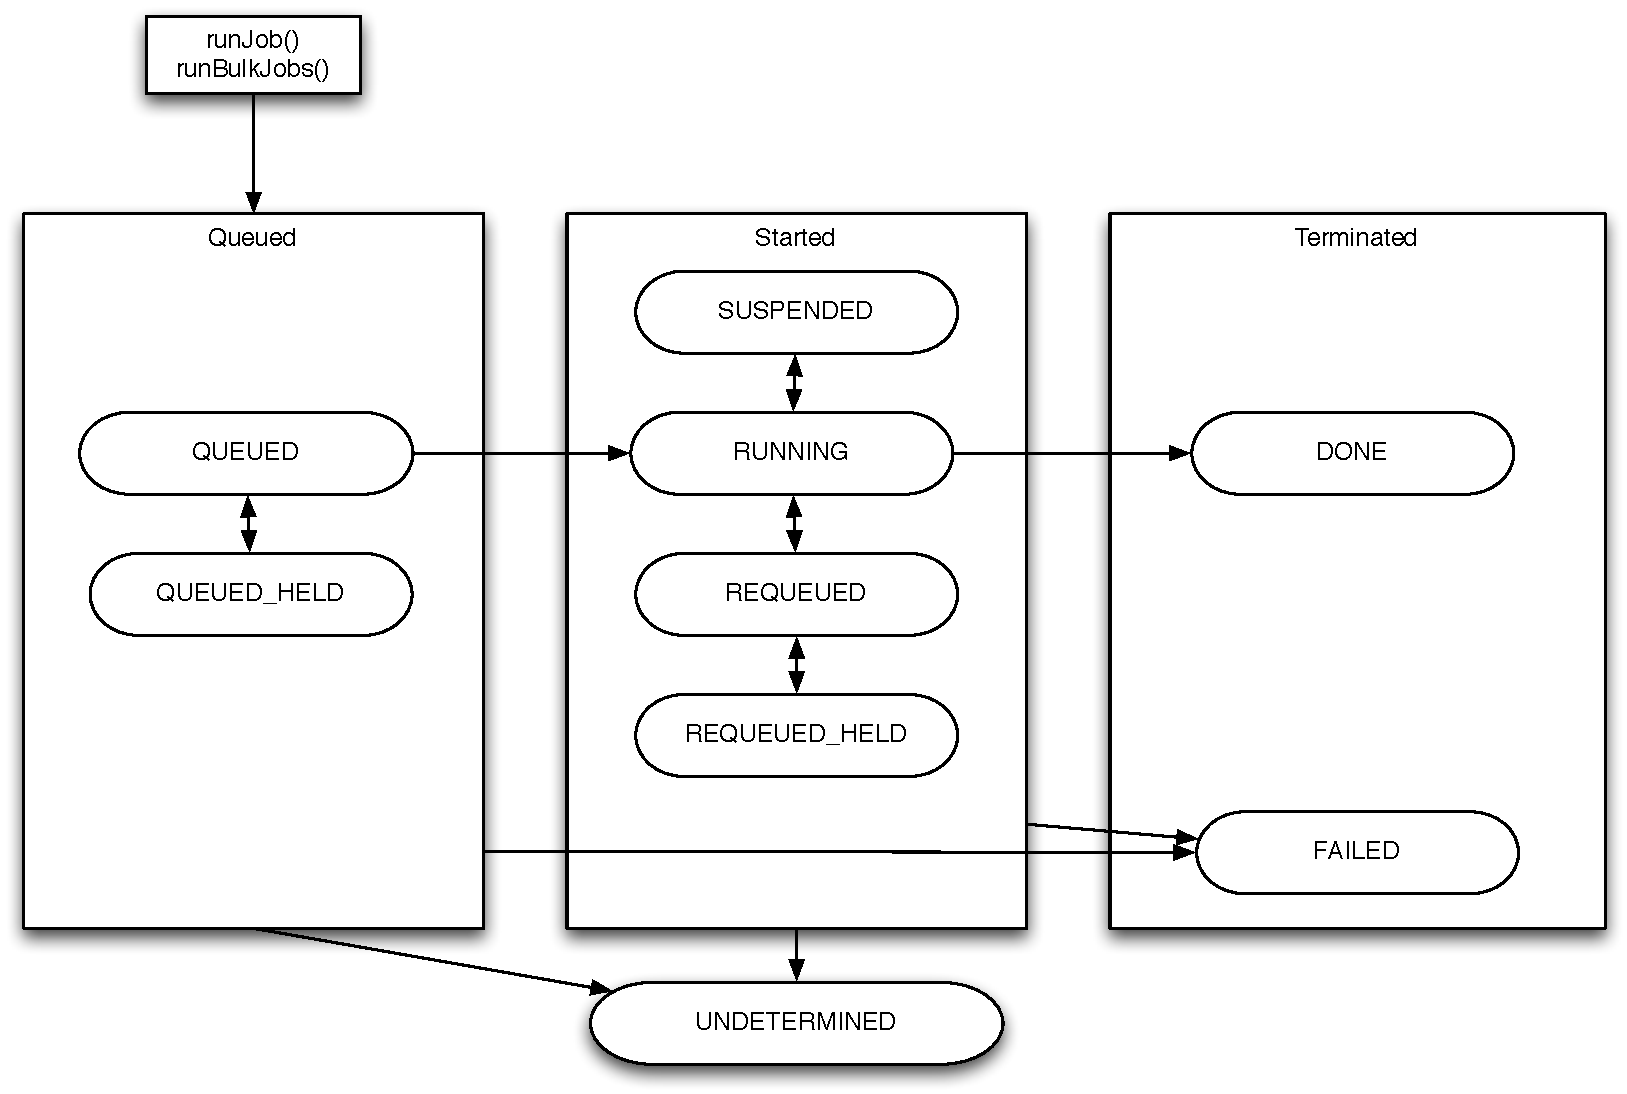
\includegraphics[width=0.9\textwidth]{statemodel}
\caption{DRMAA Job State Transition Model}
\label{fig:statemodel}
\end{figure}

The transition diagram in Figure \ref{fig:statemodel} expresses the classification of possible job states into \enquote{Queued}, \enquote{Started}, and \enquote{Terminated}. The \enquote{Terminated} class of states is final, meaning that no further state transition is  allowed. 

Implementations SHALL NOT introduce other job transitions (e.g., from \h{RUNNING} to \h{QUEUED}) beside the ones stated in Figure \ref{fig:statemodel}, even if they might happen in the underlying DRM system. In this case, implementations MAY emulate the necessary intermediate steps for the DRMAA-based application. 

When an application requests job state information, the implementation SHOULD also provide the \h{jobSubState} value (see Section \ref{sec:jobSubState}) to explain DRM-specific details about the job state. The value of this attribute is implementation-specific, but should be documented properly. Examples are extra states for staging phases or details on the hold reason. Implementations SHOULD define a DRMS-specific data structure for the sub-state information that can be converted to / from the data type defined by the language binding.

\langbind{
The IDL definition declares the \h{jobSubState} attribute as type \h{any}, expressing the fact that the language binding MUST map the data type to a generic language type (e.g., \emph{void*}, \emph{Object}) that keeps source code portability across DRMAA implementations, and accepts an \h{UNSET} value. 
}

The DRMAA job state model can be mapped to other high-level API state models. Table \ref{tab:statemappings} gives a non-normative set of examples. 

\begin{table}[ht]
\centering
\begin{tabularx}{\textwidth}{|X|X|X|}
\hline
DRMAA JobState & SAGA JobState \cite{saga} & OGSA-BES Job State \cite{gfd.108}\\
\hline
UNDETERMINED   & N/A                       & N/A \\
QUEUED               & Running                   & Pending (Queued) \\
QUEUED\_HELD   & Running                 & Pending (Queued)  \\
RUNNING            & Running                   & Running (Executing) \\
SUSPENDED         & Suspended                 & Running (Suspended) \\
REQUEUED          & Running                 &  Running (Queued) \\
REQUEUED\_HELD & Running                & Running (Queued) \\
DONE                     & Done                      & Finished \\
FAILED                 & Cancelled, Failed         & Cancelled, Failed \\
\hline
\end{tabularx}
\caption{Example Mapping of DRMAA Job States}
\label{tab:statemappings}
\end{table}

\rat{
Comparison to DRMAA 1.0: 

The differentiation between the system hold, user hold, and system / user hold job states was removed (conf. call Jan 20th 2009). There is only one hold state now. A job can now change its state from one of the SUSPENDED states to the QUEUED\_ACTIVE state (conf. call Jan 20th 2009, solves issue \#2788). The job state UNDETERMINED is now clearer defined. It expressed a permanent issue, meaning that the job state will not change by just waiting. Temporary problems in the detection of the job state are now expressed by the TryLaterException (conf. call Feb 5th 2009, solves issue \#2783). The description of the FAILED state was extended to support a more specific differentiation between different job failure reasons. The new subState feature allows the DRMAA implementation to provide better information, if available. There was no portable way of standardizing extended failure information in a better way. (conf. call May 12th 2009, solves issue \#5875) The different suspend job states from DRMAA1 (user suspended, system suspended, user / system suspended) are now combined into one suspend state. DRM systems with the need to express the different suspend reasons can use the new sub-state feature (conf. call Mar 5th 2010).

REQUEUED and REQUEUED\_HELD maps to RUNNING in BES, since BES does not allow a transition between Running and Pending (mailing list, APr. 2011)
}	

\subsection{JobSession Interface}
\label{sec:jobsession}

A job session instance acts as container for job instances controlled through the DRMAA API. The session methods support the submission of new jobs and the monitoring of existing jobs. The relationship between jobs and their session MUST be persisted, as described in Section \ref{sec:sessionmanager}. 

\lstinputlisting[linerange=JobSession-End]{drmaav2.idl}

\rat{
Comparison to DRMAA 1.0: The original separation between synchronize() and wait() was replaced by a complete new synchronization semantic in the API. DRMAA2 has now two methods, waitStarted() and waitTerminated(). The first waits for any state that expresses that the job was started, the second for any terminal status. Both methods are available on session level (wait for any of the given jobs to start / end) or on single job level (solves issue \#5880 and \#2838). The session-level functions implement the old DRMAA wait(SESSION\_ANY). The old synchronize() semantics are no longer directly supported - instead, the DRMAA application should use a looped \h{Job.wait... / JobSession.waitAny...} call. The result is a more condensed and responsive API, were the application can decide to keep the user informed during synchronization on a set of jobs. DRMAA library implementations should also become easier to design, since the danger of multithreading side effects inside the DRMAA API is reduced by this change. As a side effect, JOB\_IDS\_SESSION\_ANY and JOB\_IDS\_SESSION\_ALL are no longer needed. The special consideration of a partial failures during SESSION\_ALL wait activities is also no longer necessary (F2F meeting July 2009). The JobSession now allows to fetch also information about jobs that were not submitted through DRMAA (conf. call June 23th 2010).}

\subsubsection{contact}

This attribute reports the \h{contact} value that was used in the \h{SessionManager::createJobSession} call for this instance (see Section \ref{sec:sessionmanager}). If no value was originally provided, the default contact string from the implementation MUST be returned. This attribute is read-only.

\subsubsection{sessionName}

This attribute reports the session name, a value that resulted from the \h{SessionManager::createJobSession} or \h{SessionManager::openJobSession} call for this instance (see Section \ref{sec:sessionmanager}). This attribute is read-only.

\subsubsection{jobCategories}
\label{sec:jobcategorieslist}

This method provides the list of valid job category names which can be used for the \h{jobCategory} attribute in a \h{JobTemplate} instance. Further details about job categories are described in Section \ref{sec:jobcategories}.

\subsubsection{getJobs}

This method returns the set of jobs that belong to the job session. The \h{filter} parameter allows to choose a subset of the session jobs as return value. The semantics of the \h{filter} argument are explained in Section \ref{sec:jobinfo}. If no job matches or the session has no jobs attached, the method MUST return an empty set. If \h{filter} is \h{UNSET}, all session jobs MUST be returned.

Time-dependent effects of this method, such as jobs no longer matching to filter criteria on evaluation time, are implementation-specific. The purpose of the filter parameter is to keep scalability with a large number of jobs per session. Applications therefore must consider the possibly changed state of jobs during their evaluation of the method result.

\rat{We are aware of the fact that the automated reaping of terminated jobs in some DRM systems might change this methods result. However, there was no way to demand some standardized behavior for that.}

\subsubsection{getJobArray}

This method returns the \h{JobArray} instance with the given ID. If the session does not / no longer contain the according job array, \h{InvalidArgumentException} SHALL be thrown.

\rat {
June 2011 conf. call decided to not support JobArray filtering in the session at this point. The face-to-face meeting in June 2011 identified that DRM systems typically do not support the identification of bulk jobs in the system, so it would be hard to implement the according reporting function.
}

\subsubsection{runJob}

The \h{runJob} method submits a job with the attributes defined in the given job template instance. The method returns a \h{Job} object that represents the job in the underlying DRM system. Depending on the job template settings, submission attempts may be rejected with an \h{InvalidArgumentException}. The error details SHOULD provide further information about the attribute(s) responsible for the rejection.

When this method returns a valid \h{Job} instance, the following conditions SHOULD be fulfilled:

\begin{itemize}
	\item The job is part of the persistent state of the job session.
	\item All non-DRMAA and DRMAA interfaces to the DRM system report the job as being submitted to the DRM system.
	\item The job has one of the DRMAA job states.
\end{itemize}	

\subsubsection{runBulkJobs}
\label{sec:runbulkjobs}

The \h{runBulkJobs} method creates a set of parametric jobs, each with attributes as defined in the given job template instance. Each job in the set has the same attributes, except for the job template attributes that include the \h{PARAMETRIC\_INDEX} macro. 

If any of the resulting parametric job templates is not accepted by the DRM system, the method call MUST raise an \h{InvalidArgumentException}. No job from the set SHOULD be submitted in this case.

The first job in the set has an index equal to the \h{beginIndex} parameter of the method call. The smallest valid value for \h{beginIndex} is 1. The next job has an index equal to \h{beginIndex + step}, and so on. The last job has an index equal to \h{beginIndex + n * step}, where n is equal to\h{(endIndex - beginIndex) / step}. The index of the last job may not be equal to \h{endIndex} if the difference between \h{beginIndex} and \h{endIndex} is not evenly divisible by \h{step}. The \h{beginIndex} value must be less than or equal to \h{endIndex}, and only positive index numbers are allowed, otherwise the method SHOULD raise an \h{InvalidArgumentException}. 

Jobs can determine their index number at run time by the mechanism described in Section \ref{sec:drmaaindex}. 

The \h{maxParallel} parameter allows to specify how many of the bulk job's instances are allowed to run in parallel on the utilized resources. Implementations MAY consider this value if the DRM system supports such functionality, otherwise the parameter MUST be silently ignored.  If given, the support MUST be expressed by the \h{DrmaaCapability::BULK\_JOBS\_MAXPARALLEL} capability flag (see Section \ref{sec:drmaacapability}). If the parameter value is \h{UNSET}, no limit SHOULD be applied.

The \h{runBulkJobs} method returns a \h{JobArray} (see Section \ref{sec:jobarray}) instance that represents the set of \h{Job} objects created by the method call under a common array identity. For each of the jobs in the array, the same conditions as for the result of \h{runJob} SHOULD apply. 

\rat{
There was a discussion (mailing list Jan 2011) about having specialized job templates for bulk submission, with support for the start / end index and a slots limit. We rejected that, since job templates are intended for re-usage. 

The May 4th 2011 conf call identified Grid Engine, Torque and LSF as the only systems having support for maxParallel. The feature was determined as critical enough for still adding it, therefore the ignorance rule and the MAY semantics are applied.
}

\subsubsection{waitAnyStarted / waitAnyTerminated}
\label{sec:waitanystarted}

The \h{waitAnyStarted} method blocks until any of the jobs referenced in the \h{jobs} parameter entered one of the \enquote{Started} states. The \h{waitAnyTerminated} method blocks until any of the jobs referenced in the \h{jobs} parameter entered one of the \enquote{Terminated} states (see Section \ref{sec:jobstates}). If the input list contains jobs that are not part of the session, the method SHALL fail with an \h{InvalidArgumentException}. 

The \h{timeout} argument specifies the desired waiting time for the state change. The constant value \h{INFINITE_TIME} MUST be supported to get an indefinite waiting time. The constant value \h{ZERO_TIME} MUST be supported to express that the method call SHALL return immediately. A number of seconds can be specified to indicate the maximum waiting time . If the method call returns because of timeout, an \h{TimeoutException} SHALL be raised. 

An application waiting for some condition to happen in \emph{all} jobs of a set is expected to perform looped calls of these waiting functions. 

\rat{
People typically ask for the waitAll..() counterparts of these functions. Since they are so easy to implement in the application itself, we could not see any benefit in adding them. Due to their intended long-blocking operation, the DRM system would no be able to offer any better (meaning much faster) implementation to be wrapped by DRMAA.

A section on synchronization of multi-threaded parallel wait calls was removed. This would complicate DRMAA implementations, since synchronization does not map to the obvious state polling approach. An optimization like this would be classically a task of application-oriented APIs - so, Andre has to solve it.
}

\subsection{DrmaaCallback Interface}
\label{sec:drmaacallback}

The \h{DrmaaCallback} interface allows the DRMAA library or the DRM system to inform the application about relevant events in an asynchronous fashion. One expected use case is continuous monitoring of job state transitions. The implementation MAY decide to not deliver all events occurring in the DRM system. The support for such callback functionality is optional, indicated by the \h{DrmaaCallback::CALLBACK} flag. Also, all implementations MUST define the \h{DrmaaCallback} interface type as given in the language binding, regardless of the support for these functions.

\lstinputlisting[linerange=DrmaaCallback-End]{drmaav2.idl}
\lstinputlisting[linerange=DrmaaNotification-End]{drmaav2.idl}
\lstinputlisting[linerange=DrmaaEvent-End]{drmaav2.idl}

The application implements a \h{DrmaaCallback} interface as pre-condition for using this functionality. This interface is registered through the \h{SessionManager::registerEventNotification} method (see Section \ref{sec:sessionmanager}). On notification, the implementation or the DRM system pass a \h{DrmaaNotification} instance to the application. Implementations MAY extend this structure for further information (see Section \ref{sec:structextension}). All given information SHOULD be valid at least at the time of notification generation. 

The \h{DrmaaNotification::jobState} attribute expresses the state of the job at the time of notification generation. 

The \h{DrmaaEvent} enumeration defines standard event types for notification:

\begin{description}
	\item[NEW\_STATE] The job entered a new state, which is described in the \h{jobState} attribute. 
	\item[MIGRATED] The job was migrated to another execution host, and is now in the state described by \h{jobState}.
	\item[ATTRIBUTE\_CHANGE] A monitoring attribute of the job, such as the memory consumption, changed to a new value. The \h{jobState} attribute MAY have the value UNSET on this event.
\end{description}

DRMAA implementations SHOULD protect themselves from unexpected behavior of the called application. This includes indefinite delays or unexpected exceptions from the callee on notification processing. The implementation SHOULD prevent a nested callback at the time of occurrence, and MAY decide to deliver the according events at a later point in time. 

Scalability issues of the notification facility are out of scope for this specification. Implementations MAY support non-standardized throttling configuration options.

\rat{
We intentionally did not add \h{subState} to the notification information, since this would make callback interface implementations specific for the DRM system, without any chance for creating a portable DRMAA application. 

The \h{DrmaaNotification} structure intentionally avoids to reference a \h{Job} object - instead, all relevant lookup information (session name + job ID) is provided. This demands only non-interface data types to be understandable in the callback target. Also, it hopefully helps to support scalability of high-frequent event callbacks.
}


\subsection{Job Interface}
\label{sec:job}

Every job in the \h{JobSession} is represented by its own instance of the \h{Job} interface. It allows one to instruct the DRM system of a job status change, and to query the properties of the job in the DRM system. Implementations MAY provide \h{Job} objects for jobs created outside of a DRMAA session.

\lstinputlisting[linerange=Job-End]{drmaav2.idl}

\rat{
In comparison to DRMAA v1.0, DRMAA2 replaces the identification of jobs by strings with Job objects. This enables a tighter integration of job meta-data and identity, for the price of reduced performance in (so far not existing) DRMAA RPC scenarios. The former DRMAA control() with the JobControlAction structure is now split up into dedicated functions (such as hold() and release()) on the Job object.
	
Even though the DRMAAv2 surveys showed interest in interactive job support, this feature was intentionally left out. Reasons are the missing support in some major DRM systems, and the lack of a relevant DRMAA-related use case (conf. call Jan 7th 2010)

Issue \#5877 (support for direct job signaling) was rejected, even though there was an according request from the SAGA WG. Issue \#2782 (change attributes of submitted, but pending jobs) was rejected based on group decision.
}

\subsubsection{jobId}

This attribute reports the job identifier assigned by the DRM system in text form. This method is expected to be used as a fast alternative to the fetching of a complete \h{JobInfo} instance.

\subsubsection{sessionName}

This attribute reports the name of the \h{JobSession} that was used to create the job. If the session name cannot be determined, for example since the job was created outside of a DRMAA session, the attribute SHOULD be \h{UNSET}.

\rat{June 29th 2011 conf call decided to return session names instead of session objects. This keeps the consistent approach that instantiated session objects represent a live ``connection'' to the DRMS. Connecting to the referenced session is then a separate explicit step in the application. It also supports better that people create instances from jobs created outside of a DRMAA session.
}

\subsubsection{jobTemplate}

This attribute provides a reference to a \h{JobTemplate} instance that has equal values to the one that was used for the job submission creating this \h{Job} instance.

For jobs created outside of a DRMAA session, implementations MUST also return a \h{JobTemplate} instance here, which MAY be empty or only partially filled.
 
\subsubsection{suspend / resume / hold / release / terminate}
\label{sec:jobcontrolfunctions}

The job control functions allow modifying the status of a single job in the DRM system, according to the state model presented in Section \ref{sec:jobstates}. 

The \h{suspend} method triggers a transition from \h{RUNNING} to \h{SUSPENDED} state. 

The \h{resume} method triggers a transition from \h{SUSPENDED} to \h{RUNNING} state. 

The \h{hold} method triggers a transition from \h{QUEUED} to \h{QUEUED_HELD}, or from \h{REQUEUED} to \h{REQUEUED_HELD} state. 

The \h{release} method triggers a transition from \h{QUEUED_HELD} to \h{QUEUED}, or from \h{REQUEUED_HELD} to \h{REQUEUED} state. 

The \h{terminate} method triggers a transition from any of the \enquote{Started} states to one of the \enquote{Terminated} states. 

If the job is in an inappropriate state for the particular method call, it MUST raise an \h{InvalidStateException}.

The methods SHOULD return after the action has been acknowledged by the DRM system, but MAY return before the action has been completed. Some DRMAA implementations MAY allow these methods to be used to control jobs submitted externally to the DRMAA session. Examples are jobs submitted by other DRMAA sessions, in other DRMAA implementations, or jobs submitted via native utilities. This behavior is implementation-specific.

\subsubsection{getState}

This method allows the application to get the current status of the job according to the DRMAA state model, together with an implementation specific sub state (see Section \ref{sec:jobstates}). It is intended as a fast alternative to the fetching of a complete \h{JobInfo} instance. The timing conditions are described in Section \ref{sec:jobinfo}.

\rat{
The getState() function now also returns job subState information. This is intended as additional information for the given DRMAA job state, and can be used for expressing the hold state differentiation from DRMAA 1.0 (conf. call Mar 31st 2009).
}

\subsubsection{getInfo}

This method returns a \h{JobInfo} instance for the particular job, under the conditions described in Section \ref{sec:jobinfo}. 

\subsubsection{waitStarted / waitTerminated}

The \h{waitStarted} method blocks until the job entered one of the \enquote{Started} states. The \h{waitTerminated} method blocks until the job entered one of the \enquote{Terminated} states (see Section \ref{sec:jobstates}). All other behavior MUST work as described in Section \ref{sec:waitanystarted}.

\subsection{JobArray Interface}
\label{sec:jobarray}

 An instance of the \h{JobInfo} interface represents a set of jobs created by one operation. In DRMAA, \h{JobArray} instances are only created by the \h{runBulkJobs} method (see Section \ref{sec:jobsession}). \h{JobArray} instances differ from the \h{JobList} data structure due to their potential for representing a DRM system concept, while \h{JobList} is a DRMAA-only concept realized by language binding support.

Implementations SHOULD realize the \h{JobArray} functionality as wrapper for DRM system job arrays, if available. If the DRM system has only single job support or incomplete job array support with respect to the DRMAA-provided functionality, implementations MUST offer the \h{JobArray} functionality on their own, for example based on looped activities with a list of jobs.

\lstinputlisting[linerange=JobArray-End]{drmaav2.idl}

\rat{
We are aware of the fact that some systems (e.g., LSF at the time of writing) do not support all DRMAA control methods offered for job arrays. Since we intended to avoid optional DRMAA methods wherever we could, the text here mandates the implementation to simulate the array support on its own. For example, looping over all jobs in the array and calling \enquote{suspend} for each one is trivial to implement and fulfills the same purpose.
} 

\subsubsection{jobArrayId}

This attribute reports the job identifier assigned to the job array by the DRM system in text form. If the DRM system has no job array support, the implementation MUST generate a system-wide unique identifier for the result of the \h{runBulkJobs} method.

\subsubsection{jobs}

This attribute provides the list of jobs that are part of the job array, regardless of their state. 

\rat{
We were asked for offering a filter support similar to JobSession here. This was rejected by discussion on the list (Jan 2011), since the number of jobs returned here is normally comparatively short. In this case, the DRM system cannot provide any benefit over the looped check in the application itself.

The disappearance of terminated jobs is intentionally not specified (see discussion above for \h{getJobs}).
}

\subsubsection{sessionName}

This attribute states the name of the \h{JobSession} that was used to create the bulk job represented by this instance. If the session name cannot be determined, for example since the bulk job was created outside of a DRMAA session, the attribute SHOULD have an \h{UNSET} value.

\rat{June 29th 2011 conf call decided to return session names instead of session objects. This keeps the consistent approach that instantiated session objects represent a live ``connection'' to the DRMS. Connecting to the referenced session is then a separate explicit step in the application. It also supports better that people create instances from bulk jobs created outside of a DRMAA session.
}

\subsubsection{jobTemplate}

This attribute provides a reference to a \h{JobTemplate} instance that has equal values to the one that was used for the job submission creating this \h{JobArray} instance. 

\rat{
The use case from SAGA perspective is that the user can easily resubmit the same job - just changing for example some command line parameter, but leaving the remainder fixed (mail by Andre Merzky, July 29th 2010).  
}

\subsubsection{suspend / resume / hold / release / terminate}

The job control functions allow modifying the status of the job array in the DRM system, with the same semantic as in the \h{Job} interface (see Section \ref{sec:jobcontrolfunctions}). If one of the jobs in the array is in an inappropriate state for the particular method, the method MAY raise an \h{InvalidStateException}.

The methods SHOULD return after the action has been acknowledged by the DRM system for all jobs in the array, but MAY return before the action has been completed for all of the jobs. Some DRMAA implementations MAY allow this method to be used to control job arrays created externally to the DRMAA session. This behavior is implementation-specific.

\rat{We were asked to make explicit that some of these functions may not be atomic. However, this holds for most methods, and is not supported to be a part of the API standard.}

\subsection{Indirect environment variables}
\label{sec:drmaaindex}

DRMAA implementations SHOULD implicitly set the environment variables \h{DRMAA\_INDEX\_VAR} and \h{DRMAA\_JOB\_ID} for each job submitted to the DRM system. 

One possible implementation strategy is the transparent addition of environment variable specifications during job submission. Such a definition SHOULD NOT be visible for the application as part of the job template. If the application defines environment variables with the same name, they SHOULD override the default value. 

The \h{DRMAA\_INDEX\_VAR} environment variable MUST contain the name of the DRM system environment variable that provides the parametric index of the job being executed. Examples are \h{TASK\_ID} in GridEngine, \h{PBS\_ARRAYID} in Torque, or \h{LSB\_JOBINDEX} in LSF. For DRM systems that do not provide such an environment variable,  \h{DRMAA\_INDEX\_VAR} SHOULD not be set. If the job is not a bulk job,  \h{DRMAA\_INDEX\_VAR} SHOULD not be set.

The \h{DRMAA\_JOB\_ID} environment variable MUST contain the name of the DRM system environment variable that provides the unique identifier of the job being executed.  For DRM systems that do not provide such an environment variable,  \h{DRMAA\_JOB\_ID} SHOULD not be set. 

\rat{The Dec. 7th 2011 conf call decided upon the addition of the JOB\_ID environment variable.}

\section{Working with Advance Reservation}

Advance reservation is a DRM system concept that allows the reservation of execution resources for jobs to be submitted in the future. DRMAA encapsulates such functionality of a DRM system with the interfaces and data structures described in this chapter.

DRMAA implementations for a DRM system that does not support advance reservation MUST still implement the described interfaces, in order to keep source code portability for DRMAA-based applications. All methods related to advance reservation MUST raise an \h{UnsupportedOperationExeption} in this case. Support for advance reservation is expressed by the \h{DrmaaCapability::ADVANCE\_RESERVATION} flag (see Section \ref{sec:drmaacapability}). 

\subsection{ReservationSession Interface}
\label{sec:reservationsession}

Every \h{ReservationSession} instance acts as container for advance reservations in the DRM system. Every \h{Reservation} instance SHALL belong only to one \h{ReservationSession} instance. 

\lstinputlisting[linerange=ReservationSession-End]{drmaav2.idl}

\subsubsection{contact}

This attribute reports the \h{contact} value that was used in the \h{createReservationSession} call for this instance (see Section \ref{sec:sessionmanager}). If no value was originally provided, the default contact string from the implementation MUST be returned. This attribute is read-only.

\subsubsection{sessionName}

This attribute reports the name of the session that was used for creating or opening this \h{Reservation} instance  (see Section \ref{sec:sessionmanager}). This attribute is read-only.

\subsubsection{getReservation}

This method returns the \h{Reservation} instance that has the given \h{reservationId}. Implementations MAY support access to reservations created outside of a DRMAA session scope, under the same regularities as for the \h{MonitoringSession::getAllReservations} method (see Section \ref{sec:getallreservations}). If no reservation matches, the method SHALL raise an \h{InvalidArgumentException}.  Time-dependent effects of this method are implementation-specific. 

\subsubsection{requestReservation}

The \h{requestReservation} method SHALL request an advance reservation in the DRM system as described by the \h{ReservationTemplate}. On a successful reservation, the method returns a \h{Reservation} instance that represents the advance reservation in the underlying DRM system.

If the current user is not authorized to create reservations, \h{DeniedByDrmsException}  SHALL be raised. If the reservation cannot be performed by the DRM system due to invalid \h{ReservationTemplate} attributes, or if the demanded combination of resources is not available, \h{InvalidArgumentException} SHALL be raised. The exception SHOULD provide further details about the rejection cause in the extended error information (see Section \ref{sec:exceptions}).

Some of the requested conditions might be not fulfilled after the reservation was successfully created, for example due to execution host outages. In this case, the reservation itself SHOULD remain valid. A job using such a reservation may spend additional time in one of the non-\h{RUNNING} states. In this case, the \h{JobInfo::jobSubState} information SHOULD inform about this situation.

\rat{In DRMAA 2.0 we do not have an explicit state model for advance reservations, as the reservation state can be easily deducted by comparing current time with reservation start and end time. For this reason, we use the subState approach for informing the user about the described situation. }

\subsubsection{getReservations}

This method returns the list of reservations successfully created so far in this session, regardless of their start and end time. The list of \h{Reservation} instances is only cleared in conjunction with the destruction of the actual session instance through \h{SessionManager::destroyReservationSession} (see Section \ref{sec:sessionmanager}).

\subsection{Reservation Interface}
\label{sec:reservation}

The \h{Reservation} interface represents attributes and methods available for an advance reservation successfully created in the DRM system.  Implementations MAY offer \h{Reservation} instances for advance reservations created outside of a DRMAA session.

\lstinputlisting[linerange=Reservation-End]{drmaav2.idl}


\subsubsection{reservationId}
\label{sec:reservationid}

The \h{reservationId} is an opaque string identifier for the advance reservation. If the DRM system has identifiers for advance reservations, this attribute SHOULD provide the according value. If not, the DRMAA implementation MUST generate a value that is unique in time and extend of the DRM system.

\subsubsection{sessionName}

This attribute states the name of the \h{ReservationSession} that was used to create the advance reservation instance. If the session name cannot be determined, for example since the reservation was created outside of a DRMAA session, the attribute SHOULD have an \h{UNSET} value.

\rat{June 29th 2011 conf call decided to return session names instead of session objects. This keeps the consistent approach that instantiated session objects represent a live ``connection'' to the DRMS. Connecting to the referenced session is then a separate explicit step in the application. It also supports better that people create instances from reservation created outside of a DRMAA session.
}

\subsubsection{reservationTemplate}

This attribute provides a reference to a \h{ReservationTemplate} instance that has equal values to the one that was used to create this reservation. For reservations created outside of a DRMAA session, implementations MUST also return a \h{ReservationTemplate} instance, which MAY be empty or only partially filled.

\subsubsection{getInfo}
This method returns a \h{ReservationInfo} instance under the conditions described in Section \ref{sec:reservationinfo}. The method SHOULD throw \h{InvalidArgumentException} if the reservation is already expired (i.e., its end time passed), or if it was previously terminated. 

\subsubsection{terminate}

This method terminates the advance reservation represented by this \h{Reservation} instance. All jobs submitted with a reference to this reservation SHOULD be terminated by the DRM system or the implementation, regardless of their current state.

\section{Monitoring the DRM System}

The monitoring support in DRMAA focusses on the investigation of resources and on global data maintained by the DRM system. Session-related information is available from the \h{JobSession} and \h{ReservationSession} instances, respectively.

\subsection{MonitoringSession Interface}
\label{sec:monitoringsession}

The \h{MonitoringSession} interface provides a set of stateless methods for fetching information about the DRM system and the DRMAA implementation itself.

\lstinputlisting[linerange=MonitoringSession-End]{drmaav2.idl}

All returned data SHOULD be related to the current user running the DRMAA-based application. For example, the \h{getAllQueues} function MAY be reduced to only report queues that are usable or generally accessible for the DRMAA application and the user performing the query. 

Because of cases where such a list reduction may demand excessive overhead in the DRMAA implementation, an unreduced or only partially reduced result MAY also be returned. The behavior of the DRMAA implementation in this regard should be clearly documented. In all cases, the list items MUST be valid input for job submission or advance reservation through the DRMAA API, but MAY lead to later exceptions.

\subsubsection{getAllReservations}
\label{sec:getallreservations}

This method returns the list of all advance reservations visible for the user running the DRMAA-based application. In contrast to a \h{ReservationSession::getReservations} call, this method SHOULD also return reservations that were created outside of DRMAA (e.g., through command-line tools) by this user. 

 The DRM system or the DRMAA implementation is at liberty to restrict the set of returned reservations based on site or system policies, such as security settings or scheduler load restrictions. The returned list MAY contain reservations that were created by other users. It MAY also contain reservations that are not usable for the user.

This method SHALL raise an \h{UnsupportedOperationException} if advance reservation is not supported by the implementation.

\subsubsection{getAllJobs}

This method returns the list of all DRMS jobs visible to the user running the DRMAA-based application. In contrast to a \h{JobSession::getJobs} call, this method SHOULD also return jobs that were submitted outside of DRMAA (e.g., through command-line tools) by this user. The returned list MAY also contain jobs that were submitted by other users if the security policies of the DRM system allow such global visibility. The DRM system or the DRMAA implementation is at liberty, however, to restrict the set of returned jobs based on site or system policies, such as security settings or scheduler load restrictions.

Querying the DRM system for all jobs might result in returning an excessive number of \h{Job} objects. Implications to the library implementation are out of scope for this specification. 

The method supports a \h{filter} argument for fetching only a subset of the job information available. Both the return value semantics and the filter semantics SHOULD be similar to the ones described for the \h{JobSession::getJobs} method (see Section \ref{sec:jobsession}). 

\langbind{
Language bindings SHOULD NOT try to solve the scalability issues by replacing the sequence type of the return value with some iterator-like solution. This approach would break the basic snapshot semantic intended for this method.
}

\rat{
The non-argumentation about the scalability problem was the final result of a clarification attempt. We hand this one over to the implementors. (conf call Jul 14th 2010)
}

\subsubsection{getAllQueues}

This method returns a list of queues available for job submission in the DRM system. The names from all \h{QueueInfo} instances in this list SHOULD be a valid input for the \h{JobTemplate::queueName} attribute (see Section \ref{sec:queuename}). The result can be an empty list or might be incomplete, based on queue, host, or system policies. It might also contain queues that are not accessible for the user at job submission time because of queue configuration limits.

The \h{names} parameter supports restricting the result to \h{QueueInfo} instances that have one of the names given in the argument. If the \h{names} parameter value is \h{UNSET}, all \h{QueueInfo} instances should be returned.

\subsubsection{getAllMachines}

This method returns the list of machines available in the DRM system as execution host. The returned list might be empty or incomplete based on machine or system policies. The returned list might also contain machines that are not accessible for the user, e.g., because of host configuration limits.

The \h{names} parameter supports restricting the result to \h{MachineInfo} instances that have one of the names given in the argument. If the \h{names} parameter value is \h{UNSET}, all \h{MachineInfo} instances should be returned.

\section{Complete DRMAA IDL Specification}
\label{sec:idl}

The following text shows the complete IDL specification for the DRMAAv2 application programming interface. The ordering of IDL constructs here has no normative meaning, but ensures an easier compilation with a standard CORBA IDL compiler for syntactical correctness checks. This demands also some additional forward declarations to resolve circular dependencies.

\lstinputlisting[linerange=Module-End]{drmaav2.idl}
\lstinputlisting[linerange=JobState-End]{drmaav2.idl}
\lstinputlisting[linerange=OperatingSystem-End]{drmaav2.idl}
\lstinputlisting[linerange=CpuArchitecture-End]{drmaav2.idl}
\lstinputlisting[linerange=ResourceLimitType-End]{drmaav2.idl}
\lstinputlisting[linerange=DrmaaEvent-End]{drmaav2.idl}
\lstinputlisting[linerange=DrmaaCapability-End]{drmaav2.idl}
\lstinputlisting[linerange=DataTypes-End]{drmaav2.idl}
\lstinputlisting[linerange=JobInfo-End]{drmaav2.idl}
\lstinputlisting[linerange=SlotInfo-End]{drmaav2.idl}
\lstinputlisting[linerange=ReservationInfo-End]{drmaav2.idl}
\lstinputlisting[linerange=JobTemplate-End]{drmaav2.idl}
\lstinputlisting[linerange=ReservationTemplate-End]{drmaav2.idl}
\lstinputlisting[linerange=DrmaaNotification-End]{drmaav2.idl}
\lstinputlisting[linerange=QueueInfo-End]{drmaav2.idl}
\lstinputlisting[linerange=Version-End]{drmaav2.idl}
\lstinputlisting[linerange=MachineInfo-End]{drmaav2.idl}
\lstinputlisting[linerange=Exception-End]{drmaav2.idl}
\lstinputlisting[linerange=DrmaaReflective-End]{drmaav2.idl}
\lstinputlisting[linerange=DrmaaCallback-End]{drmaav2.idl}
\lstinputlisting[linerange=ReservationSession-End]{drmaav2.idl}
\lstinputlisting[linerange=Reservation-End]{drmaav2.idl}
\lstinputlisting[linerange=JobArray-End]{drmaav2.idl}
\lstinputlisting[linerange=JobSession-End]{drmaav2.idl}
\lstinputlisting[linerange=Job-End]{drmaav2.idl}
\lstinputlisting[linerange=MonitoringSession-End]{drmaav2.idl}
\lstinputlisting[linerange=SessionManager-End]{drmaav2.idl}
\lstinputlisting[linerange=ModuleEnd-End]{drmaav2.idl}

\section{Security Considerations}
\label{sec:security}

The DRMAA API does not specifically assume the existence of a particular security infrastructure in the DRM system. The scheduling scenario described herein presumes that security is handled at the point of interaction with the DRM system. It is assumed that credentials owned by the application using the API are in effect for the DRMAA implementation too, so that it acts as stakeholder for the application. 

An authorized but malicious user could use a DRMAA implementation or a DRMAA-enabled application to saturate a DRM system with a flood of requests. Unfortunately for the DRM system, this case is not distinguishable from the case of an authorized good-natured user who has many jobs to be processed. For temporary load defense, implementations SHOULD utilize the \h{TryLaterException}, if possible. In case of permanent issues, the implementation SHOULD raise the \h{DeniedByDrmsException}.

DRMAA implementers SHOULD guard their product against buffer overflows that can be exploited through DRMAA enabled interactive applications or portals. Implementations of the DRMAA API will most likely require a network to coordinate subordinate DRM system requests. However, the API makes no assumptions about the security posture provided by the networking environment. Therefore, application developers SHOULD also consider the security implications of \enquote{on-the-wire} communications in this case.

For environments that allow remote or protocol based DRMAA clients, the implementation SHOULD offer support for secure transport layers to prevent man in the middle attacks. 

\section{Contributors}


The DRMAA working group is grateful to numerous colleagues for support and discussions on the topics covered in this document, in particular (in alphabetical order, with apologies to anybody we have missed): 

Guillaume Alleon, 
Ali Anjomshoaa, 
Ed Baskerville, 
Harald Böhme, 
Nadav Brandes,
Matthieu Cargnelli, 
Karl Czajkowski, 
Piotr Domagalski, 
Fritz Ferstl, 
Paul Foley, 
Nicholas Geib, 
Becky Gietzel, 
Alleon Guillaume, 
Daniel S. Katz,
Andreas Haas,
Tim Harsch, 
Greg Hewgill, 
Rayson Ho, 
Eduardo Huedo, 
Dieter Kranzmüller, 
Krzysztof Kurowski, 
Peter G. Lane, 
Miron Livny, 
Ignacio M. Llorente, 
Martin v. Löwis, 
Andre Merzky, 
Thijs Metsch,
Ruben S. Montero, 
Greg Newby, 
Steven Newhouse, 
Michael Primeaux, 
Greg Quinn, 
Hrabri L. Rajic,
Martin Sarachu, 
Jennifer Schopf, 
Enrico Sirola, 
Chris Smith, 
Ancor Gonzalez Sosa, 
Douglas Thain, 
John Tollefsrud, 
Jose R. Valverde, 
and Peter Zhu.

Special thanks must go to Andre Merzky, who participated as SAGA working group representative in numerous DRMAA events. 

This specification was developed by the following core members of the DRMAA working group at the Open Grid Forum:

\begin{samepage}
\textbf{Roger Brobst}\\
Cadence Design Systems, Inc.\\
555 River Oaks Parkway \\
San Jose, CA 95134, United States\\
Email: rbrobst@cadence.com\\  

\textbf{Daniel Gruber}\\
Univa GmbH\\
c/o Rüter und Partner\\
Prielmayerstr. 3\\
80335 München, Germany\\
Email: dgruber@univa.com\\

\textbf{Mariusz Mamoński}\\
Poznań Supercomputing and Networking Center\\
ul. Noskowskiego 10\\
61-704 Poznań, Poland\\
Email: mamonski@man.poznan.pl\\ 

\textbf{Daniel Templeton} \\
Cloudera Inc.\\
210 Portage Avenue\\
Palo Alto, CA 94306, United States\\
Email: daniel@cloudera.com\\

\textbf{Peter Tröger (Corresponding Author)} \\
Hasso Plattner Institute at University of Potsdam \\
Prof.-Dr.-Helmert-Str. 2-3 \\
14482 Potsdam, Germany \\
Email: peter@troeger.eu \\
\end{samepage}

%%%%%%%%%%%%%%%%%%%%%%%%%%%%%%%%%%%%%%%%%%%%%%%%%%%%%%%%%%%%%%%%%%%%%%%%%%%%%%%%%%%%
%%% Insert content above this line
%%%%%%%%%%%%%%%%%%%%%%%%%%%%%%%%%%%%%%%%%%%%%%%%%%%%%%%%%%%%%%%%%%%%%%%%%%%%%%%%%%%%


\section{Intellectual Property Statement}

 The OGF takes no position regarding the validity or scope of any
 intellectual property or other rights that might be claimed to
 pertain to the implementation or use of the technology described in
 this document or the extent to which any license under such rights
 might or might not be available; neither does it represent that it
 has made any effort to identify any such rights.  Copies of claims of
 rights made available for publication and any assurances of licenses
 to be made available, or the result of an attempt made to obtain a
 general license or permission for the use of such proprietary rights
 by implementers or users of this specification can be obtained from
 the OGF Secretariat.

 The OGF invites any interested party to bring to its attention any
 copyrights, patents or patent applications, or other proprietary
 rights which may cover technology that may be required to practice
 this recommendation.  Please address the information to the OGF
 Executive Director.


\section{Disclaimer}

 This document and the information contained herein is provided on an
 ``As Is'' basis and the OGF disclaims all warranties, express or
 implied, including but not limited to any warranty that the use of
 the information herein will not infringe any rights or any implied
 warranties of merchantability or fitness for a particular purpose.


\section{Full Copyright Notice}

 Copyright \copyright \ Open Grid Forum (\copyrightyears). Some Rights
 Reserved.

 This document and translations of it may be copied and furnished to
 others, and derivative works that comment on or otherwise explain it
 or assist in its implementation may be prepared, copied, published
 and distributed, in whole or in part, without restriction of any
 kind, provided that the above copyright notice and this paragraph are
 included as references to the derived portions on all such copies and
 derivative works. The published OGF document from which such works
 are derived, however, may not be modified in any way, such as by
 removing the copyright notice or references to the OGF or other
 organizations, except as needed for the purpose of developing new or
 updated OGF documents in conformance with the procedures defined in
 the OGF Document Process, or as required to translate it into
 languages other than English. OGF, with the approval of its board,
 may remove this restriction for inclusion of OGF document content for
 the purpose of producing standards in cooperation with other
 international standards bodies. 

 The limited permissions granted above are perpetual and will not be
 revoked by the OGF or its successors or assignees. 


% \phantomsection\addcontentsline{toc}{section}{References}
\section{References}
\renewcommand{\refname}{}
\vspace*{-3em}
\bibliography{bibliography}

\newpage
\appendix
\section{Errata (September 2012)}
\label{sec:errata}

The following changes were applied in the September 2012 revision of this document:

\subsection*{Section 3}

\h{HOME\_DIRECTORY}, \h{WORKING_DIRECTORY} and \h{PARAMETRIC_INDEX} are now native string constants, instead of being a separate enumeration.

\subsection*{Section 4.1}

The term \h{TRUE64} was changed to \h{TRU64} at four occasions.

\subsection*{Section 4.2}

The enumeration of CPU architectures was extended with the following entries:

\h{ARM64, PARISC64, MIPS64} 

The description of the CPU architectures was improved and extended with the new architectures .
Table 3 was accordingly extended with entries for ARM64, PARISC64 and MIPS64. The JSDL mappings are the same as for the 32-bit counterparts of these architectures.

\subsection*{Section 4.3}

\h{DATA\_SEG\_SIZE} was renamed to \h{DATA\_SIZE} at two occasions.

The description of this attribute was modified in the following way:

\begin{itemize}
\item \emph{DATA\_SIZE:} The maximum amount of memory the job can allocate for initialized data, uninitialized data and heap space, in kilobyte.
\end{itemize}

\subsection*{Section 5.7.25}

\h{DATA\_SEG\_SIZE} was renamed to \h{DATA\_SIZE}.
 
\subsection*{Section 8.2.7}

The following two sentences were removed without replacement:

\begin{quote}
\emph{The largest (syntactically) allowed value for endIndex MUST be defined by the language binding.}

\emph{Further restrictions on the maximum endIndex MAY be implied by the implementation.}
\end{quote} 
 
\subsection*{Section 8.4}

The return type of \h{waitStarted} and \h{waitTerminated} was changed from \h{Job} to \h{void}. 
 
\subsection*{Section 11}

The term \h{TRUE64} was changed to \h{TRU64}. \h{DATA\_SEG\_SIZE} was renamed to \h{DATA\_SIZE}. 

The enumeration \h{CpuArchitecture} was extended with the entries \h{ARM64}, \h{PARISC64} and \h{MIPS64}.

The return type of \h{waitStarted} and \h{waitTerminated} was changed from \h{Job} to \h{void}. 

\end{document}


%This pages hosts the DRMAA proposals for standardized configuration names. It is unlikely that this list ends up in the real specification - instead, we intend to maintain it on drmaa.org as \enquote{working group recommendation}. Implementations shall be never mandated to support any of this.

%All attributes are expected to work on the execution host.

%The April 14th DRMAA telco concluded that the group should only specify the configuration name suggestions, since installation aspects are truly site-specific.

%Configuration Name	 Source	 Description	 Expected Environment Variables	 Expected Binaries in Path	 Expected Libraries in LD_LIBRARY_PATH	 Expected Files
%MPI	 GFD.115	 Any MPI environment	 ??	 mpirun	 ??	 ??
%GridMPI	 GFD.115	 GridMPI environment	 ??	 ??	 ??	 ??
%IntelMPI	 GFD.115	 Intel MPI environment	 ??	 ??	 ??	 ??
%LAM-MPI	 GFD.115	 LAM/MPI environment	 ??	 ??	 ??	 ??
%MPICH1	 GFD.115	 MPICH Version 1 environment	 ??	 ??	 ??	 ??
%MPICH2	 GFD.115	 MPICH Version 2 environment	 ??	 ??	 ??	 ??
%MPICH-GM	 GFD.115	 MPICH-GM environment	 ??	 ??	 ??	 ??
%MPICH-MX	 GFD.115	 MPICH-MX environment	 ??	 ??	 ??	 ??
%MVAPICH	 GFD.115	 MVAPICH (MPI-1) environment	 ??	 ??	 ??	 ??
%MVAPICH2	 GFD.115	 MVAPICH2 (MPI-2) environment	 ??	 ??	 ??	 ??
%OpenMPI	 GFD.115	 Open MPI environment	 ??	 ??	 ??	 ??
%POE	 GFD.115	 POE (IBM MPI) environment	 ??	 ??	 ??	 ??
%PVM	 GFD.115	 Parallel Virtual Machine environment	 ??	 ??	 ??	 ??
%OpenMP	 DRMAA WG	 OpenMP ennvironment	 OMP_NUM_THREADS	 ??	 ??	 ??
%Java	 DRMAA WG	 Java environment	 JAVA_HOME	 java, javacc	 ??	 ??%
